% Copyright (C) 2001, International Business Machines
% Corporation, Ted Ralphs and others. All Rights Reserved.

\documentclass[openany,twoside,11pt]{book}

\setlength{\parindent}{0in}
\setlength{\parskip}{0.15in}
\setlength{\oddsidemargin}{0.5in}
\setlength{\evensidemargin}{0in}
\setlength{\topmargin}{0in}
\setlength{\textwidth}{6in}

\usepackage{mathenv}
\usepackage{graphicx}
%\usepackage{epsfig}

\newcommand{\be}{\begin{enumerate}}
\newcommand{\ee}{\end{enumerate}}
\newcommand{\bc}{\begin{center}}
\newcommand{\ec}{\end{center}}
\newcommand{\bt}{\begin{tabular}}
\newcommand{\et}{\end{tabular}}
\newcommand{\bd}{\begin{description}}
\newcommand{\ed}{\end{description}}
\newcommand{\bi}{\begin{itemize}}
\newcommand{\ei}{\end{itemize}}
\newcommand{\bv}{\begin{verbatim}}
\newcommand{\ev}{\end{verbatim}}
\newcommand{\functiondef}[1]{\subsubsection{#1}}

\renewcommand{\functiondef}[1]{\item[\Large $\triangleright$] {\bf \Large #1}}
\newcommand{\describe}{\item[Description:] \hfill}
\newcommand{\args}{\item[Arguments:] \hfill}
\newcommand{\returns}{\item[Return values:] \hfill}
\newcommand{\postp}{\item[Post-processing:] \hfill}
\newcommand{\nopostp}{\item[Post-processing:] None \hfill}

\newcommand{\BB}{{\sc COIN/BCP}}
\newcommand{\TM}{{\sc TreeManager}}
\newcommand{\LP}{{\sc LP}}
\newcommand{\ra}{$\rightarrow$}

\newcommand{\eqsep}{\hspace{.25em}}
\newcommand{\commentout}[1]{}
\newcommand{\code}[1]{{\tt #1}}

\begin{document}

\title{\BB\ User's Manual}
\author{
T.K. Ralphs\thanks{Department of Industrial and Manufacturing Systems 
Engineering, Lehigh University, Bethlehem, PA 18015, {\tt
tkralphs@lehigh.edu}, {\tt http://www.lehigh.edu/\~{ }tkr2}} 
\and
L. Lad\'anyi\thanks{Department of Mathematical Sciences, 
IBM T.J. Watson Research Center, Yorktown Heights,
NY 10598} \\
}
\date{January 2001}
\maketitle

\newpage

\thispagestyle{empty}

\vspace*{3in}
\begin{center}
{\copyright 2001 International Business Machines Corporation, Ted
Ralphs and others. All right reserved.}
\end{center}

\newpage

\tableofcontents

%%%%%%%%%%%%%%%%%%%%%%%%%%%%%%%%%%%%%%%%%%%%%%%%%%%%%%%%%%%%%%%%%%%%%%%%%%%%%%
% Insert here the references that are not referred to anywhere, but we want
% them to be listed anyway.
%%%%%%%%%%%%%%%%%%%%%%%%%%%%%%%%%%%%%%%%%%%%%%%%%%%%%%%%%%%%%%%%%%%%%%%%%%%%%%

\begin{tabbing}
%\cite{B:ahuja-magnanti-orlin} \kill
%\cite{B:cook-lovasz-seymour} \kill
\end{tabbing}

%%%%%%%%%%%%%%%%%%%%%%%%%%%%%%%%%%%%%%%%%%%%%%%%%%%%%%%%%%%%%%%%%%%%%%%%%%%%%%

\chapter{Introduction}
\label{man-intro}
%===========================================================================%
%                                                                           %
% This file is part of the documentation for the SYMPHONY MILP Solver.      %
%                                                                           %
% SYMPHONY was jointly developed by Ted Ralphs (tkralphs@lehigh.edu) and    %
% Laci Ladanyi (ladanyi@us.ibm.com).                                        %
%                                                                           %
% (c) Copyright 2000-2008 Ted Ralphs. All Rights Reserved.                  %
%                                                                           %
% SYMPHONY is licensed under the Common Public License. Please see          %
% accompanying file for terms.                                              %
%                                                                           %
%===========================================================================%

\section{Introducing SYMPHONY \VER}
\label{whats-new}

Welcome to the SYMPHONY Version \VER\ user's manual. Whether you are a new
user or simply upgrading, this manual will help you get started with what we
hope you will find to be a useful and powerful framework for solving
mixed-integer linear programs (MILP) sequentially or in parallel. The
subroutines in the \BB\ library comprise a state-of-the-art MILP solver with a
modular design that makes it easy to customize for various problem settings.
SYMPHONY works out of the box as a generic MILP solver that can be invoked
from the command line, through an interactive shell, or by linking to the
provided callable library, which has both C and C++ interfaces with a look and
feel similar to that of other popular solvers (see Sections \ref{C_Interface}
and \ref{C++_Interface} for the library routines). Models can be read in MPS
or GMPL (a subset of AMPL) format, as well as by interfacing with more
powerful modeling environments, such as FlopC++ (also provided with the
distribution). To develop a customized SYMPHONY application, various callbacks
can be written and parameters set that modify the default behavior of the
algorithm. Section~\ref{callback} contains an overview of the API for these
subroutines. Files containing function stubs are provided with the
distribution.

SYMPHONY can be built on almost any platform and can be configured either for
serial computation or in a wide variety of parallel modes. The parallel
version can be built for either a fully distributed environment (network of
workstations) or a shared-memory environment simply by changing a few
configuration options (see Chapter~\ref{getting_started}). To run in a
distributed environment, the user must have installed the {\em
\htmladdnormallink{Parallel Virtual Machine}{http://www.ccs.ornl.gov/pvm/}}
(PVM), available for free from Oak Ridge National Laboratories. To run in a
shared-memory environment, the user must have installed an OpenMP compliant
compiler (gcc 4.2 is currently the only compiler tested and fully supported).

\section{What's New}

For what's new in Version \VER, please check the \texttt{README}
file that comes with the distribution.

\section{A Brief History}
\label{history}

Since the inception of optimization as a recognized field of study in
mathematics, researchers have been both intrigued and stymied by the
difficulty of solving many of the most interesting classes of discrete
optimization problems. Even combinatorial problems, though conceptually easy
to model as integer programs, have long remained challenging to solve in
practice. The last two decades have seen tremendous progress in our ability to
solve large-scale discrete optimization problems. These advances have
culminated in the approach that we now call {\it branch and cut}, a technique
(see \cite{Grotschel84cut,padb:branc,hoff:LP}) which brings the computational
tools of branch and bound algorithms together with the theoretical tools of
polyhedral combinatorics. Indeed, in 1998, Applegate, Bixby, Chv\'atal, and
Cook used this technique to solve a {\em Traveling Salesman Problem} instance
with 13,509 cities, a full order of magnitude larger than what had been
possible just a decade earlier \cite{concorde} and two orders of magnitude
larger than the largest problem that had been solved up until 1978. This feat
becomes even more impressive when one realizes that the number of variables in
the standard formulation for this problem is approximately the {\em square} of
the number of cities. Hence, we are talking about solving a problem with
roughly {\em 100 million variables}.

There are several reasons for this impressive progress. Perhaps the most
important is the dramatic increase in available computing power over the last
decade, both in terms of processor speed and memory. This increase in the
power of hardware has subsequently facilitated the development of increasingly
sophisticated software for optimization, built on a wealth of theoretical
results. As software development has become a central theme of optimization
research efforts, many theoretical results have been ``re-discovered'' in
light of their new-found computational importance. Finally, the use of
parallel computing has allowed researchers to further leverage their gains.

Because of the rapidly increasing sophistication of computational techniques,
one of the main difficulties faced by researchers who wish to apply these
techniques is the level of effort required to develop an efficient
implementation. The inherent need for incorporating problem-dependent methods
(most notably for dynamic generation of variables and cutting planes) has
typically required the time-consuming development of custom implementations.
Around 1993, this led to the development by two independent research groups of
software libraries aimed at providing a generic framework that users could
easily customize for use in a particular problem setting. One of these groups,
headed by J\"unger and Thienel, eventually produced ABACUS (A Branch And CUt
System) \cite{abacus1}, while the other, headed by the authors, produced what
was then known as COMPSys (Combinatorial Optimization Multi-processing
System). After several revisions to enable more broad functionality, COMPSys
became SYMPHONY (Single- or Multi-Process Optimization over Networks). A
version of SYMPHONY written in C++, which we call COIN/BCP has also been
produced at IBM under the COIN-OR project \cite{coin-or}. The COIN/BCP package
takes substantially the same approach and has the same functionality as
SYMPHONY, but has extended SYMPHONY's capabilities in some areas.

\section{Related Work}
\label{related}

The 1990's witnessed a broad development of software for discrete
optimization. Almost without exception, these new software packages were based
on the techniques of branch, cut, and price. The packages fell into two main
categories---those based on general-purpose algorithms for solving
mixed-integer linear programs (MILPs) (without the use of special structure)
and those facilitating the use of special structure by interfacing with
user-supplied, problem-specific subroutines. We will call packages in this
second category {\em frameworks}. There have also been numerous
special-purpose codes developed for use in particular problem settings.

Of the two categories, MILP solvers are the most common. Among the dozens of
offerings in this category are MINTO \cite{MINTO}, MIPO \cite{MIPO}, bc-opt
\cite{bc-opt}, and SIP \cite{SIP}. Generic frameworks, on the other hand, are
far less numerous. The three frameworks we have already mentioned (SYMPHONY,
ABACUS, and COIN/BCP) are the most full-featured packages available. Several
others, such as MINTO, originated as MILP solvers but have the capability of
utilizing problem-specific subroutines. CONCORDE \cite{concorde, concorde2}, a
package for solving the {\em Traveling Salesman Problem} (TSP), also deserves
mention as the most sophisticated special-purpose code developed to date.

Other related software includes several frameworks for implementing parallel
branch and bound. Frameworks for general parallel branch and bound include
PUBB \cite{PUBB}, BoB \cite{BoB}, PPBB-Lib \cite{PPBB-Lib}, and PICO
\cite{PICO}. PARINO \cite{PARINO} and FATCOP \cite{chen:fatcop2} are parallel
MILP solvers.

\section{How to Use This Manual}

The manual is divided into six chapters. The first is the introduction, which
you are reading now. Chapter \ref{getting_started} describes how to install
SYMPHONY from either a source or binary distribution. If you have already
managed to get SYMPHONY running using the instructions in the \code{README}
file, you might want to skip to Chapter~\ref{API-overview}. However, keep in
mind that the manual contains additional details for customizing your build.
Chapter \ref{API-overview} contains an overview of how to use in all three
major modes---as a black-box solver through the interactive shell or on the
command line, as a callable library, and as a customizable framework. Chapter
\ref{SYMPHONY-design} contains further depth and a more complete technical
description of the design and implementation of SYMPHONY. In Section
\ref{design}, we describe the overall design of SYMPHONY without reference to
the implementational details and with only passing reference to parallelism.
In Section \ref{modules}, we discuss the details of the implementation. In
Section \ref{parallelizing}, we briefly discuss issues involved in parallel
execution of SYMPHONY. Chapter \ref{SYMPHONY-development} describes in detail
how to develop a custom application using SYMPHONY. Note that it is not
necessary to read Chapter \ref{SYMPHONY-design} before undertaking development
of a SYMPHONY application, but it may help. Chapter \ref{SYMPHONY-reference}
contains reference material. Section \ref{C_Interface} contains a description
of the native C interface for the callable library. Section
\ref{C++_Interface} contains a description of the interface for C++
environments. Section \ref{API} contains a description of the user callback
functions. SYMPHONY's parameters are described in Section \ref{params}. For
reference use, the HTML version of this manual may be more practical, as the
embedded hyperlinks make it easier to navigate.

\section{Getting Additional Help}
\label{resources}

The main point of entry for additional help, trouble-shooting, and
problem-solving is the SYMPHONY Wiki and development Web site at
\begin{center}
\url{https://projects.coin-or.org/SYMPHONY}
\end{center}
There, bug reports can be submitted by clicking on the ``New Ticket'' button
and also previous bug reports searched. For general questions, there is also a
\BB\ user's mailing list. To subscribe, visit
\begin{center}
\url{http://list.coin-or.org/mailman/listinfo/coin-symphony}
\end{center}





\chapter{Getting Started: Sample Compiling}
\label{getting-started}
% Copyright (C) 2001, International Business Machines
% Corporation, Ted Ralphs and others. All Rights Reserved.

Having familiarized yourself with the overall design of \BB\ in
Chapter \ref{man-intro}, you are now ready to get started with using
\BB\ to develop applications of your own. The remainder of this manual
is contains the technical details you need to successfully undertake
this task. This chapter provides a description of how to get started
with \BB. This is basically the same information contained in the
README file that comes with the distribution.

Although \BB\ is inherently intended to be compiled and run on
multiple architectures and across distributed networks, for now we do not
use GNU's autoconf. The make files are designed to conveniently
allow builds for multiple architectures within a single directory
tree. This means that there may be a little hand configuring to do and you
might need to know a little about your computing environment in order
to make \BB\ compile. This should be limited to editing the make files
and providing some path names. You may also have to live with some
complaints from the compiler because of missing function prototypes,
etc.

\section{System Requirements}

Currently, to obtain and compile \BB, you need to be running some
version of Unix, preferably with the gcc/g++ compiler installed.
Before you try to compile \BB, you should first ensure that the
version of gcc/g++ you are using is at least 2.95.1 by typing {\tt gcc -v}
on the command line. If you have an earlier version, \BB\ may not
compile correctly -- ask your sysadmin for an upgrade. If you're lucky
enough to be your own sysadmin, then you're probably running Linux.
The default version that comes with some Linux distributions, such as
Redhat 6.2, is earlier than 2.95.1 so you should download and install a later
version. This may also involve upgrading some other packages on which
gcc depends.

There are a few auxiliary applications that you might also want to
have installed. If you want to use CVS to download the code and update
it automatically (highly recommended), then you should also install or
ask for CVS to be installed. If you are unsure of what CVS is, please
visit {\tt www.cvs.org}. If you choose not to use CVS, then
you can download the code as a tar file. The applications {\tt tkcvs} and 
{\tt tkdiff} provide a nice graphical interface to {\tt cvs}. Finally, if
you download {\tt doxygen} ({\tt www.doxygen.org}) and {\tt qt} 
({\tt www.trolltech.com}), you will be able to automatically generate very
nice documentation from the Bcp source code in an HTML format.

\section{Obtaining the Source Code}

\subsection{Using CVS}

To obtain the source code using CVS: 
\begin{itemize}
\item Set the {\tt CVSROOT} environment variable to be \\
{\tt :pserver:anonymous@oss.software.ibm.com:/usr/cvs/coin}
\item Issue {\tt cvs login} command with password {\tt anonymous} 
\item Issue {\tt cvs checkout MODULE} where {\tt MODULE} is one of
\begin{itemize}
\item {\tt Bcp}: branch, cut, and price framework,
\item {\tt Bcp-all}: BCP framework plus Osi and Vol
\item {\tt Mkc}: multiple knapsack with color constraints (application),
\item {\tt MaxCut}: Maximum weighted cut (application),
\item {\tt mkc7}: large sample mps file for Mkc, 
\item {\tt Vol}: volume algorithm, 
\item {\tt Cgl}: cut generator library,
\item {\tt Osi}: open solver interface, 
\item {\tt Dfo}: derivative free optimization,
\item {\tt COIN}: to get all modules,
\end{itemize}
\end{itemize}

If you are just starting with Bcp, get the module {\tt Bcp-all}. It will
automatically get the two sample applications ({\tt Mkc} and {\tt MaxCut}),
as well as the other necessary modules ({\tt Osi} and {\tt Vol}). Note that
the directory {\tt COIN/} will be installed as a subdirectory of
whatever directory you issue the CVS commands from. The simplest thing
to do is to issue the commands from your home directory and then enter
the subdirectory {\tt COIN/} to work with the source files.

\subsection{Downloading a {\tt tar} File}

The tar files can be obtained from {\tt www.coin-or.org}. Simply
download the latest files and unpack them in your home directory.
This will create a {\tt COIN/} subdirectory, if one does not already
exist, and place the source files in subdirectories of this directory.
These files follow the same naming scheme as the CVS modules.

Note that the files in the repository have {\tt .tar.gz} extension 
indicating that the archive file has been compressed using {\tt gzip}. On 
U*ix systems use gunzip to uncompress them first, on Windows Winzip can
uncompress and unpack the archive.

\section{Initial compilation and testing}

Since the whole project lives in the {\tt COIN} directory in the rest of this
section every path specified is relative to this directory.

\begin{itemize}
\item First, edit the file {\tt Makefiles/Makefile.location}. This file 
   contains definitions for which libraries you want to build and
   the location of libraries that might be needed (e.g., zlib to read
   compressed MPS files). Set the following variables as needed.
  \begin{itemize}
  \item {\tt CoinDir}: to the path to the {\tt COIN/} directory
  \item Uncomment lines that add support for different libraries 
    such as libz, and different LP solvers.
  \item Set the paths for the added libraries. 
  \end{itemize}
\item You should not need to make any modifications to 
  {\tt Bcp/Makefile}. 
\item Now, edit the application specific make file. This
  is {\tt Examples/MaxCut/Makefile.maxcut} for the MaxCut example. 
  Here are the variables that you can set:
  \begin{itemize}
  \item {\tt USER\_OPT}: options the compiler should use
    for compiling the user's code.
  \item {\tt COMM\_PROTOCOL}: which message-passing
    protocol to use. Currently the options are {\tt PVM} and {\tt NONE}
    (compile as a serial application). 
  \item {\tt USER\_SRC\_PATH}: a list of directories (besides {\tt TM}, 
    {\tt LP}, etc. -- see Section \ref{source-files} for the directory
    structure) the user has source codes in.
  \end{itemize}
\item In addition, you will see that there are some other
  variables to set once you have written your own application. These
  include paths to your source files and the names of your source files.
  We will discuss how to construct this make file in more detail later
  in the manual. 
\end{itemize}
        
\subsection{Compiling for serial execution}

As mentioned above, {\tt COMM\_PROTOCOL} must be set to {\tt NONE} in the user
application Makefile. 

\begin{itemize}
\item First you have to create the volume library (if you plan to use the
  volume algorithm as your LP engine):
  \begin{itemize}
  \item Change directory into {\tt Faa/Vol} and type {\tt make}
  \end{itemize}
\item Create the Osi library:
  \begin{itemize}
  \item Change directory into {\tt Osi} and type {\tt make}
  \end{itemize}
\item Type ``{\tt make}'' in the application directory. To
  start out, we recommend that you try to compile the {\tt MaxCut}
  application in the directory {\tt Examples/MaxCut}
  application module. Dependency files will be created in 
  {\tt Bcp/dep} and in 
  {\tt Examples/MaxCut/dep}. Object files will be placed in 
  {\tt Bcp/\$(ARCH)} and in 
  {\tt Examples/MaxCut/\$(ARCH)}, where \$(ARCH) is the platform you
  run on combined with the optimization level (e.g, Linux-g or AIX-4.3-O).
  This latter directory also contains the executable named {\tt bcps} (the
  ``s'' stands for being serial).
\item To test the sample program type {\tt \$(ARCH)/bcps sample.par} on the
  command line. The sample parameter file and sample data file are included 
  in the distribution.
\end{itemize}

\subsection{Compiling for distributed networks}

To use \BB\ on a network of computers fist a message passing library must be
installed. At the moment \BB\ has an interface to the 
{\em Parallel Virtual Machine} (PVM) software only (an MPI interface is
planned). The current version of PVM can be obtained at 
{\tt www.ccs.ornl.gov/pvm}. It should compile and install without 
any problem. The user will have to set a few environment variable (such as 
{\tt PVM\_ROOT}), but this is all explained clearly in the PVM
documentation. Note that there must be a link to the compiled executable
from the {\tt \$PVM\_ROOT/bin/\$PVM\_ARCH} directory in order for
parallel processes to be spawned correctly.

The compilation procedure for \BB\ and the location of the files are almost
identical to what's described in the previous subsection with the following
differences:

\begin{itemize}
\item Set {\tt COMM\_PROTOCOL} to {\tt PVM} in the user application Makefile.
\item The executable name will be {\tt bcpp}.
\item Make a symbolic link from the
  {\tt \$(PVM\_ROOT)/bin/\$(PVM\_ARCH)/} directory 
  to the executable.
  This is required by PVM unless you override the
  default directory in your PVM hostfile.
\item Start the PVM daemon by typing ``{\tt pvm}'' on the command line
  and then typing ``{\tt quit}''.
\item To test the sample program first start up the pvm daemon on each of the
  machines you plan to use in the computation (how to do this is also
  explained in the PVM documentation) and then start \BB\ by issuing the
  {\tt \$(ARCH)/bcpp sample.par} command. The sample parameter file and 
  sample data file are included in the distribution.
\end{itemize}

Now you should have successfully compile and execute the sample application.
Once you have accomplished this much, you are well on your way to having an
application of your own. 


\chapter{Developing Applications with \BB}
\label{development}
% Copyright (C) 2001, International Business Machines
% Corporation, Ted Ralphs and others. All Rights Reserved.

\section{Directory Layout (location of the source files)}
\label{dev:source-files}

The easiest way to get oriented is to examine the organization of the
source files. Once you install the \BB\ distribution and enter the
\code{Bcp} directory, you will see several subdirectories, including
one called \code{Bcp-common/}. \code{Bcp-common/} contains the source
files for the internal framework. Users should not have to modify
these files, but should be familiar with their organization. The other
directories contain the source code for applications. There are two
samples available, a Max Cut solver (\code{MaxCut/}) and a solver for
the Multiple Knapsack Problem with Color Constraints (\code{Mkc/}).
First let's explore the Bcp-common directory.

Within \code{Bcp-common/}, there are directories associated with each
of the modules, a directory called \code{Member/} and a directory 
(\code{include/}) for the header files. The source files in \code{Member/}
contain the implementation of methods of classes that are used in
multiple modules (like cuts and variables), while the module
directories contain module specific class methods and module specific
functions.

The same directory hierarchy is used in the directories of the sample
applications and it is recommended that the user adheres to this
convention simply because the \code{Bcp/Makefile} automatically looks
for user source files in these directories. If the user places her
files in different directories then she must specify those directories
in \code{USER\_SRC\_PATH}.

\section{Overview of the Class Hierarchy}
\label{dev:overview-hierarchy}

We now briefly describe the class hierarchy from the user's point of view. Our
aim here is not to describe the full class structure, but just those parts
that the user needs to be familiar with in order to derive new user classes
and override the appropriate methods. As we discussed in Chapter
\ref{man-intro}, we have taken an object-oriented approach with the main
objects being the cuts and variables. As such, there are three main
``object'' classes from which the user may want to derive new
problem-specific descendents. These are:
\begin{itemize}
\item \code{BCP\_cut}: This class is used for describing cuts. There are three
  child classes derived from this one which implement the three
  different types of cuts---core, indexed, and algorithmic.
\item \code{BCP\_var}: This class is used for describing variables. Again,
  there 
  are three derived classes which implement the three different types
  of variables---core, indexed, and algorithmic.
\item \code{BCP\_solution}: This class is used for describing feasible
  solutions to the full problem. This description may be implemented
  simply as a list of the nonzero variables and their corresponding
  values or can be a user-defined representation of a more
  combinatorial nature. For instance, in the Traveling Salesman
  Problem, the user may wish to store feasible solutions directly as
  permutations of the nodes instead of just as a list of edge variable
  indices and values.
\end{itemize}
Ideally, these would be the only classes the user would need to worry
about. However, in order to modularize the code and support
parallelism, we have deviated from an idealized, object-oriented
design and defined some module-oriented ``interface'' classes as well.
These classes do not contain any data elements, but instead contain
methods which are unique to a particular module and cannot be
contained in one of our primary object classes. They also contain
methods which work on sets of objects---these cannot be implemented in
the standard, object-oriented fashion. As an example, all the
subroutines for communicating data between the modules. The interface
classes are:
\begin{itemize}
\item \code{BCP\_xx\_user}: Here, ``xx'' is the name of a particular module.
  The 
  user must derive a new class for each module in which she wants to
  override a default method. Note that although these base classes
  exist primarily as containers for module-specific methods, the user
  can also use his derived classes to store the problem data needed
  for performing the user-defined methods in that module.
  Alternatively, these data structures could be defined in a separate
  base class and then, using multiple inheritance, derived into a
  common child class.
\item \code{USER\_initialize}: This class contains subroutines for generating
  objects from the derived interface classes. This is also where the
  messaging environment and LP solver environment objects are created.
\end{itemize}
In addition to deriving from these classes as appropriate, the user must also
provide the definition of the function called \code{BCP\_user\_init()} which
returns an object of the 
class derived from \code{USER\_initialize}.

\section{The Flow of the Algorithm}

Keeping in mind this basic class structure, we now describe again, as
in Chapter \ref{man-intro}, the overall flow of the BCP algorithm, but
this time with more detail and an emphasis on how the interface
routines defined in the \code{BCP\_xx\_user} classes fit into this
flow. In some cases, it may be important to know the specific order in
which the interface routines are called since procedures performed in
one subroutine could depend on data generated in a previous
subroutine. This applies mainly to the LP module, which has the
largest number of associated interface routines.

%We will describe which methods the user can
%override in each module class and in which order those methods are invoked.
%This latter information is useful in case she wants to precompute something in
%one method and return results in another. For example, while testing
%feasibility she might find violated cuts she would want to report when cut
%generation is requested. Note that the user need not override all methods she
%can, indeed, for most problems she would want to override only a small
%fraction of the methods (see Table \ref{xxx}).

In Figures \ref{dev:initmodule} and \ref{dev:lploop}, 
the arrows between boxes indicate the flow
of the algorithm. Keep in mind that these charts merely give a
high-level description of the algorithm. Section
\ref{dev:user-derived} and the HTML documentation contain a full and
detailed description of the API. Figure \ref{dev:initmodule} indicates
how the solver is initialized and lists the interface routines used by
the tree manager, the cut generator, and the variable generator.
First, the solver environment is initialized (see Section
\ref{dev:USER_initialize}), then the module-specific user classes are
created. Afterwards, the user specifies the initial set of core and
extra variables and packs the problem data to be sent to the other
modules. Initialization of each of the slave processes begins with the
unpacking of these data at their destinations.

Once the solver is initialized, the TM module utilizes only three
interface methods. The first one initializes a new phase (see Section
\ref{two-phase}), the second receives a new feasible solution, while
the third compares two search tree nodes. This comparison function is
used to insert new candidate nodes into a priority queue. The top
element of the queue will be selected for processing when an LP
process becomes available. Similarly, the CG and VG modules also call
relatively few interface routines. Their only job is to wait for a
primal (dual) solution from which they try to generate violated valid
inequalities (improving columns). The generated objects are sent back
to the LP process.Figure (\ref{dev:lploop}) describes the flow of
the LP solver loop, from where the majority of the interface routines
are called. These routines will be described below.

\begin{figure}
\begin{center}
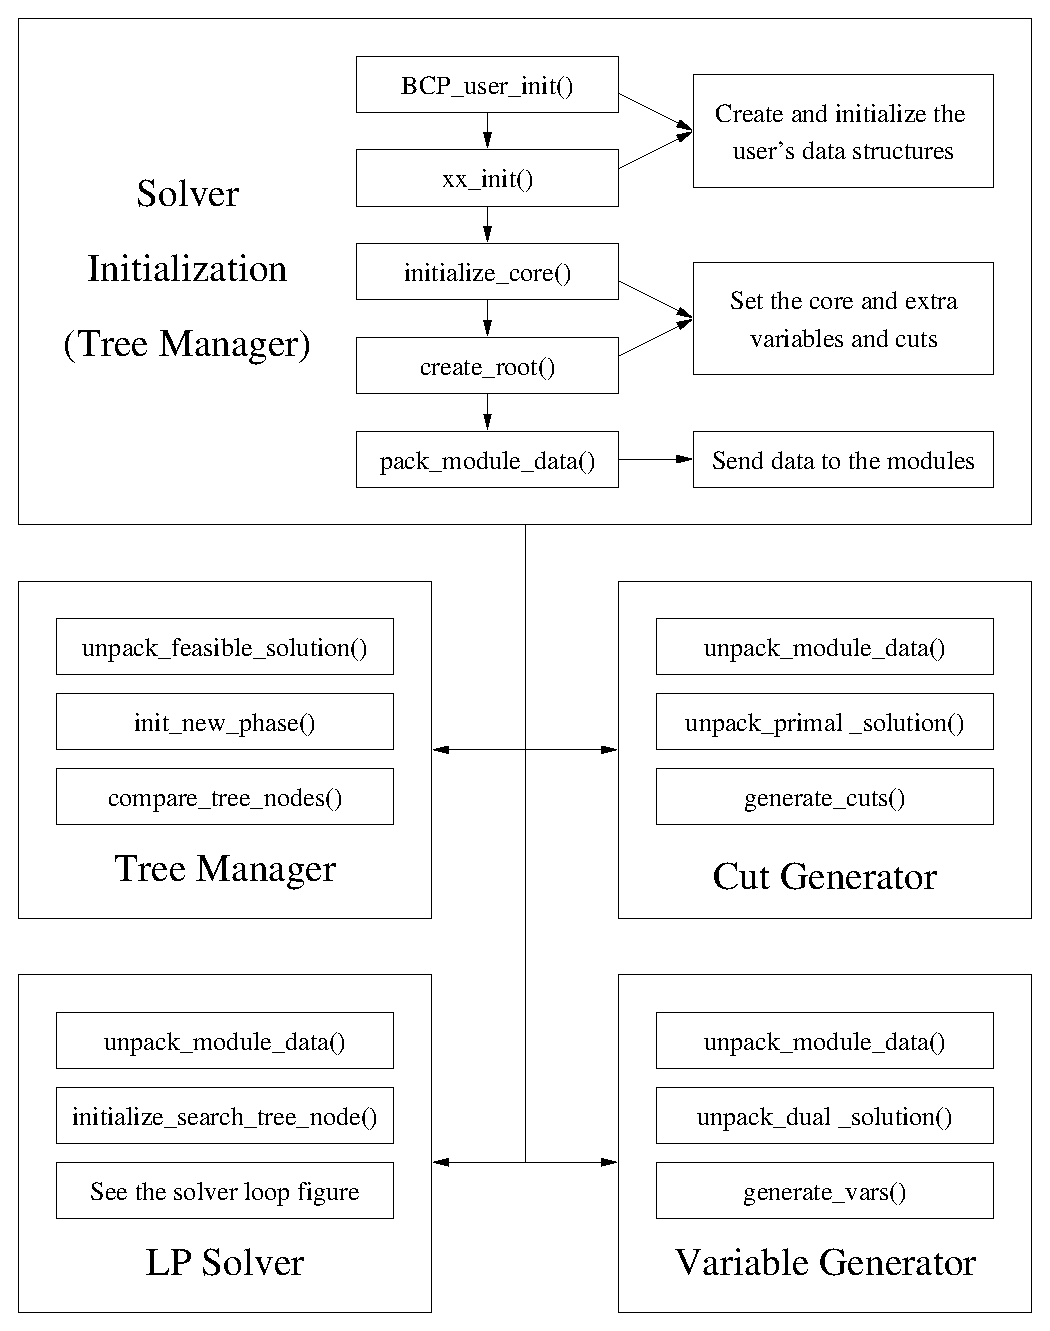
\includegraphics[scale=0.75]{flow-init.eps}
\end{center}
\caption{\label{dev:initmodule} Solver initialization and algorithm overview}
\end{figure}

\begin{figure}
\begin{center}
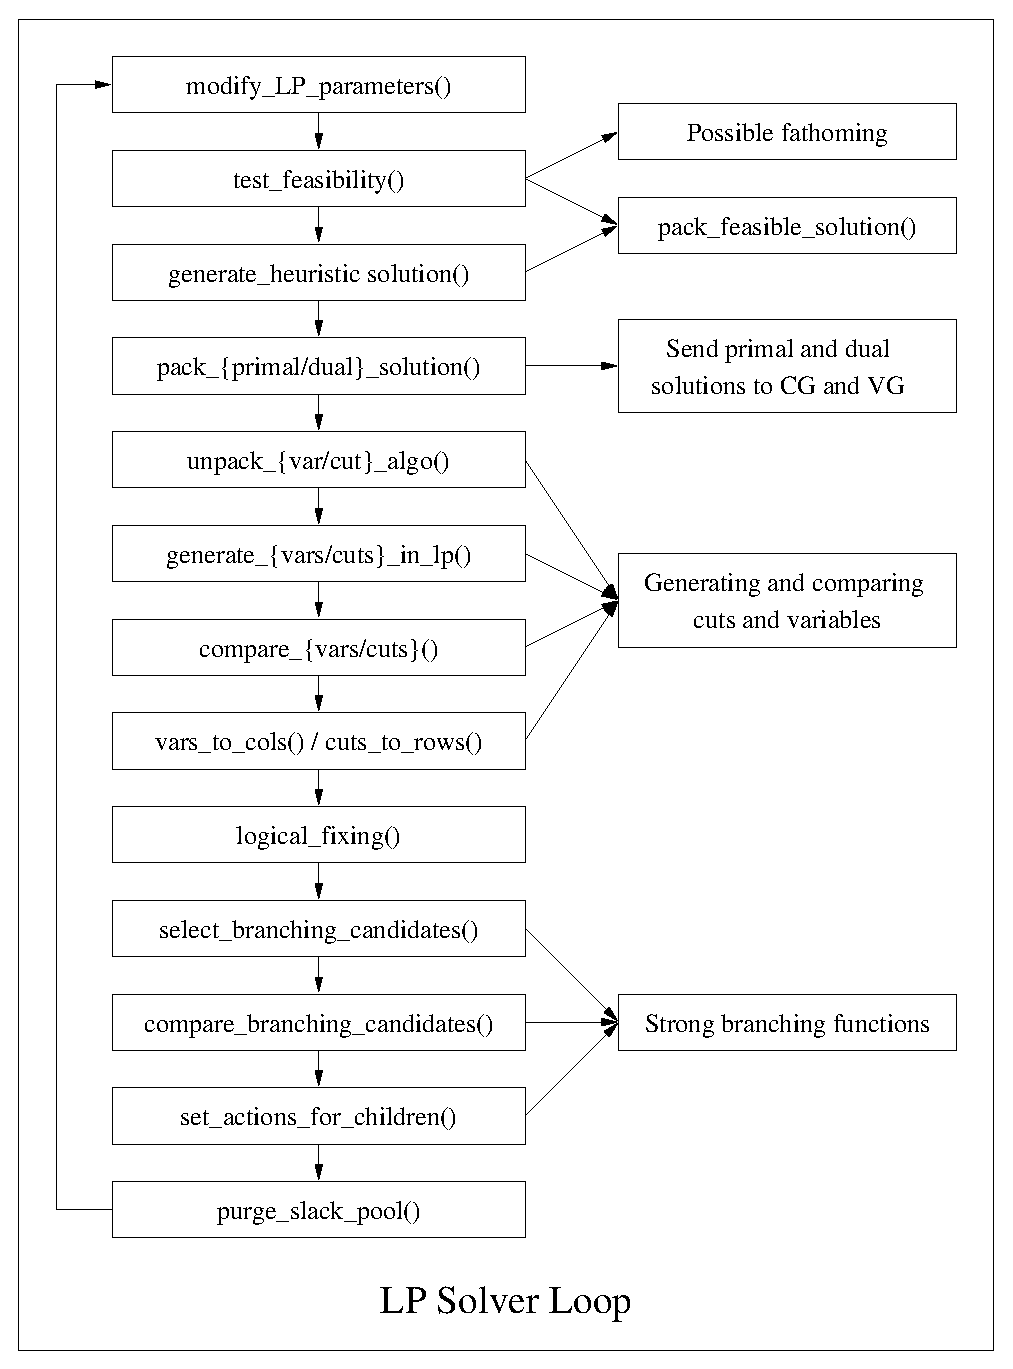
\includegraphics[scale=0.75]{flow-lploop.eps}
\end{center}
\caption{\label{dev:lploop}LP solver loop}
\end{figure}

\subsection{Fathoming procedure}

Fathoming, which is very simple
in a regular branch and cut algorithm is much more involved when
pricing is present. The reason is that introducing new columns can
push the lower bound below the global upper bound or can restore
feasibility if the LP relaxation was found infeasible. If a true
optimal solution is desired in a BCP algorithm, then a search tree
node can be fathomed if and only if there are no columns that can
restore feasibility and there is no column with negative reduced cost.
Of these two conditions the first one is the ``worse''. Almost always
there are variables that can be introduced to restore feasibility, but
usually that pushes the lower bound too high. However, we {\em must}
restore feasibility, because there can be columns with negative
reduced cost afterwards that could bring down the objective value. On
the other hand, when fathoming would happen because of too high lower
bound, all we got to look for are columns with negative reduced cost.
Frequently none are found (especially if the global upper bound is
really good) so the node can really be fathomed. For this reason it is
recommended that users wanting to generate variables on the fly set up
their model in a way that ensures primal feasibility at all times.
(Not to mention that then she doesn't have to override the feasibility
restoration methods.)

For each search tree node \BB\ maintains a state, that is, whether there are
indexed or algorithmic variables not in the formulation. Furthermore, for
indexed variables \BB\ can maintain a list about which ones have been
permanently priced out (excluded from any solution in the subtree). To utilize
this ability of \BB, only two very simple methods must be overridden:
\code{next\_indexed\_var()} and \code{create\_indexed\_var()}. The first
method is 
used to enumerate the indices of the indexed variables one by one, the second
method is used to actually create the indexed variables.

Now if fathoming would happen because the lower bound exceeds the upper bound
then, if \BB\ is instructed to maintain the above mentioned list, first the
not-yet-priced-out indexed variables are tested then the 
\code{generate\_vars\_in\_lp()} method is invoked for finding algorithmic
variables with negative reduced cost. 

If fathoming would happen because of infeasibility then again first the
indexed variables tested whether any of them destroys the proof of
infeasibility (i.e., whether it has a negative inner product with the
specified dual ray) then the \code{restore\_feasibility()} method is invoked so
that the user can test the algorithmic variables.

\section{Details of the Interface}
\label{dev:user-derived}

As mentioned earlier in our overview of the class hierarchy (Section
\ref{dev:overview-hierarchy}), the user can modify the behavior of the
framework by overriding the default methods. To override the methods
in a particular module, she simply derives a new child class from the
corresponding \code{BCP\_xx\_user} base class and overrides the
appropriate methods. If not overridden, the default method will be
invoked by the framework. Whenever possible, methods have default
which will work for the most common problem settings. In some cases,
there are several default implementations from which the user can
choose by setting a parameter. Alternatively, these methods can
be invoked directly by the user as desired, allowing for the use of
different methods in different situations. In the remainder of this
section, we describe in more detail the virtual methods of the
interface classes. These descriptions are at a high level---for the
exact specification, see the HTML manual pages included with the
distribution \cite{HTML-manual}.

\subsection{The \code{USER\_initialize} class}
\label{dev:USER_initialize}

The user must communicate the existence of the objects she designed to
\BB. For example, for all processes she intends to use she must have
derived something from the \code{BCP\_xx\_user} classes. Since \BB\
contains the \code{main()} function there are two ways to achieve this.
The ``C'' style solution is to have a functions declared in \BB\ but
not defined. These functions must be defined by the user and return
pointers to objects defined by her. The disadvantage of this solution
is that the user has to define all of these functions, even if she
doesn't intend to create some type of objects. Furthermore, if there
are possible defaults she must indicate somehow to the calling
function that a default should be executed.

\BB\ employs a C++ style coding here. Only one function is declared that the
user must define, \code{BCP\_user\_init()}. This function must
return an object of a type she derived from \code{USER\_initialize} and
in which she overrode some methods. This way the user is forced to
define only one function, and she can choose the default behavior
(like initializing the LP engine class) by simply not overriding a
method.

When \BB\ will be converted into a library there will be no need for this
class. 

\begin{itemize}
\item \code{msgenv\_init()}: return the message passing environment to be used.
  The user probably doesn't want to override this method, as the default 
  \BB\ uses will be determined by the value of \code{COMM\_PROTOCOL} in the
  application Makefile.
\item \code{tm\_init()}: return the object the user has derived from 
  \code{BCP\_tm\_user}. Note that this method should also take care of reading
  the parameter file and the problem data and whatever initialization the user
  wants to do. The user {\em must} override this method, there {\em must} be a
  user derived tree manager class.
\item \code{lp\_init()}: return the object the user has derived from 
  \code{BCP\_lp\_user}. The user {\em must} override this method, there 
  {\em must} be a user derived LP class.
\item \code{cg\_init()} and \code{vg\_init()}: return the object the user has
  derived 
  from the classes \code{BCP\_cg\_user} and \code{BCP\_vg\_user}. The user
  must override these if and only if she wants to generate cuts / variables.
\end{itemize}

\subsection{The \code{BCP\_tm\_user} class}

\begin{itemize}
\item \code{pack\_module\_data()}: in this method the user must pack the data
  that will be needed to perform computations in other modules. By default
  this method is empty and it is very likely that the user wants to override
  it.

  Note that this method should be overridden if and only if the 
  \code{unpack\_module\_data()} methods of any other process is overridden.

\item \code{unpack\_feasible\_solution()}: unpack a solution that is feasible
  to 
  the problem. Not really necessary to override, it should only be done if the
  default generic solution (\code{BCP\_solution\_generic}) format is not good
  for 
  the user for some reason. That format contains the description and value of
  all variables that are at nonzero level in the solution. The user may have a
  much more compact and intuitive representation of the solution, in which
  case she would override this method.

  By default a \code{BCP\_solution\_generic} object is unpacked.

  Note that this method should be overridden if and only if the corresponding
  method, \code{pack\_feasible\_solution()} in the class \code{BCP\_lp\_user}
  is 
  overridden.
  
\item \code{(un)pack\_warmstart()}: (un)pack warmstarting information for a
  search tree node. The user probably doesn't want to override this method, as
  it should correspond to the LP solver selected. The default, just like for
  the LP engine, will be determined by the defined \code{COIN\_USE\_XXX} value.

\item \code{(un)pack\_var\_algo()}: (un)pack an algorithmic variable. By
  default this method throws an exception since if it is invoked then the user
  must have generated an algorithmic variable in which case she must override
  this method.

\item \code{(un)pack\_cut\_algo()}: (un)pack an algorithmic cut. By
  default this method throws an exception since if it is invoked then the user
  must have generated an algorithmic cut in which case she must override
  this method.

\item \code{initialize\_core()} and \code{create\_root()}: the first of these
  two 
  methods sets up the core of the problem (see Section \ref{variables-cuts})
  while the second specifies what extra cuts and variables should be present
  in the root node. By default the first method creates an empty core and the
  second method does not list any extra objects. Therefore to get something
  into the root node the user must override at least one of them.
  
\item \code{init\_new\_phase()}: perform any necessary initialization before a
  new phase starts in the algorithm. Nothing is done as default. If the user
  does not do any pricing then the it is probably fine.  Otherwise (since the
  column generation strategy must be specified in this method, too) the user
  must override it.
  
\item \code{compare\_tree\_nodes()}: compare two search tree nodes. Return true
  if the first node should be processed before the second one. The default
  behavior is controlled by the \code{TreeSearchStrategy} parameter which is
  set to \code{BCP\_BestFirstSearch} by default. 

\end{itemize}

\subsection{The \code{BCP\_lp\_user} class}

This is by far the most complex class. 
\begin{itemize}
\item \code{unpack\_module\_data()}: unpack the data packed for this process in
  the TM by the \code{pack\_module\_data()} method. By default
  this method is empty and it is very likely that the user wants to override
  it.

  Note that if this method is overridden then the TM's
  \code{pack\_module\_data()} method must be overridden, too.

\item \code{(un)pack\_warmstart()}: (un)pack warmstarting information for a
  search tree node. The user probably doesn't want to override this method, as
  it should correspond to the LP solver selected. The default, just like for
  the LP engine, will be determined by the defined \code{COIN\_USE\_XXX} value.

\item \code{(un)pack\_var\_algo()}: (un)pack an algorithmic variable. By
  default this method throws an exception since if it is invoked then the user
  must have generated an algorithmic variable in which case she must override
  this method.

\item \code{(un)pack\_cut\_algo()}: (un)pack an algorithmic cut. By
  default this method throws an exception since if it is invoked then the user
  must have generated an algorithmic cut in which case she must override
  this method.
  
\item \code{initialize\_solver\_interface()}: return the LP engine. The user
  probably doesn't want to override this method as the default \BB\ uses will
  be determined by the defined \code{COIN\_USE\_XXX} value. However, it's
  possible that the user wants to define more than one LP solver and choose
  one based on a parameter.  In this case she needs to override this method.
  In this case she should also override the \code{(un)pack\_warmstart()}
  methods 
  in the TM and LP user classes as well.

\item \code{initialize\_new\_search\_tree\_node()}: do some preprocessing
  (e.g., 
  logical tightening of bounds on variables and/or constraints) on the
  search tree node before it gets processed. By default this method is empty.
  A good candidate for overriding in column generation methods, since there
  branching information usually encodes some logic, thus implying significant
  tightening.

\item \code{modify\_lp\_parameters()}: a chance to modify the parameters of the
  LP engine. By default this method is empty. Those experimenting with using
  different parameters in ``regular'' LP optimization and LP optimization in
  strong branching will want to override it.

\item \code{test\_feasibility()}: test whether the LP solution is feasible for
  the whole problem. If it is so then return a \code{BCP\_solution} object.
  The default just tests whether all integrality requirements are met.
  (Actually there are several default options but they differ in their speed
  only by exploiting special knowledge, e.g., knowing that all variable must
  be binary.) If the user has her own representation of the solution she
  definitely wants to override it (the default method creates a 
  \code{BCP\_solution\_generic} object). Also, she must override it if cuts are
  being generated as \BB\ has no way of knowing whether the not yet added cuts
  are all satisfied.

\item \code{generate\_heuristic\_solution()}: try to come up with a good
  solution 
  from the given LP solution. By default this method is empty. If the user has
  a quick heuristic it's worth to add it here since a good solution can
  drastically cut the size of the search tree. 

\item \code{pack\_feasible\_solution()}: the pair of
  \code{unpack\_feasible\_solution()} in the tree manager. Override neither or
  both. The default tries to treat and pack the solution argument as a 
  \code{BCP\_solution\_generic} object and throws an exception if it is not
  such a 
  solution. 
  
\item \code{pack\_primal\_solution()}: pack the information to be sent to the
  cut 
  generator (this is usually the primal solution). The default method packs a
  selected set of variables along with their values. The selection is
  parameter driven, it can be everything, the nonzeros, the fractional values,
  etc. Override neither or both of this method and its pair, 
  \code{unpack\_primal\_solution()} in the cut generator. There is no reason to
  override it if no cut generator processes are started.

\item \code{pack\_dual\_solution()}: pack the information to be sent to the
  variable generator (this is usually the dual solution). The default method
  packs a selected set of cuts along with their dual values. The selection is
  parameter driven, it can be everything, the nonzeros, the fractional values,
  etc. Override neither or both of this method and its pair, 
  \code{unpack\_dual\_solution()} in the variable generator. There is no reason
  to override it if no variable generator processes are started.

\item \code{display\_lp\_solution()}: display the result of most recent LP
  optimization. This method is invoked every time an LP relaxation is
  optimized and the user can display (or not display) it. By default the
  solution is displayed if the verbosity of \BB\ is high enough.

  This method exists mainly for debugging purposes. Few people would ever want
  to see all LP solutions. It's unlikely anyone would override this method.

\item \code{next\_indexed\_var()} and \code{create\_indexed\_var()}:
  methods used if \BB\ is to maintain the list of indexed variables that are
  permanently priced out. The first method returns the
  user index of the variable whose index is the next one after the argument
  while the second method creates an indexed variable (and the corresponding
  column) given the index.
  By default they all throw exceptions. The user must
  override them if they are to be used.

\item \code{restore\_feasibility()}:
  These methods are invoked before fathoming a search tree node that has
  been found infeasible. If \BB\ maintains the list of indexed variables that
  are permanently priced out then by the time this method is invoked every
  indexed variable is tested whether it can destroy the proof of
  infeasibility and the user should look only for algorithmic variables.
  Otherwise (i.e., if \BB\ does not maintain the list) it is up to the user to
  check both indexed and algorithmic variables whether they ``cut off'' the
  dual rays. 

\item \code{cuts\_to\_rows()}: create the corresponding rows for a set of cuts
  with 
  respect to the currently active variables. By default this method throws an
  exception (should not be called if not written). It must be overridden if
  cuts are generated.

\item \code{vars\_to\_cols()}: create the corresponding columns for a set of
  variables with respect to the currently active cuts. By default this
  method throws an exception (should not be called if not written). 
  It must be overridden if variables are generated.

\item \code{generate\_cuts\_in\_lp()}: generate cuts within the LP process.
  Sometimes too much information 
  would need to be transmitted for cut generation (e.g., the full tableau
  for Gomory cuts) or the cut generation is so fast that transmitting the
  info would take longer than generating the cuts. In such cases it might
  better to generate the cuts locally. This routine provides the opportunity.
  By default this method is empty (will be interfaced with Cgl).

\item \code{generate\_vars\_in\_lp()}: generate variables within the LP
  process. 
  Sometimes too much information 
  would need to be transmitted for variable generation or the variable
  generation is so fast that transmitting the info would take longer than
  generating the variables. In such cases it might be better to generate
  the variables locally. This routine provides the opportunity. By default
  this method is empty.

\item \code{compare\_cuts()}: compare two generated cuts. Cuts are generated in
  different iterations, 
  they come from the Cut Pool, etc. There is a very real possibility that
  the LP process receives several cuts that are either identical or one
  of them is better then another (cuts off everything the other cuts
  off). This routine is used to decide which one to keep if not both. By 
  default both cuts are kept. The user should override this method only if
  there is a significant chance that cuts will be regenerated.

\item \code{compare\_vars()}: compare two generated variables. Variables are
  generated in different 
  iterations, they come from the Variable Pool, etc. There is a very real
  possibility that the LP process receives several variables that are
  either identical or one of them is better then another (e.g., almost
  identical but has much lower reduced cost). This routine is used to
  decide which one to keep if not both. By 
  default both variables are kept. The user should override this method only
  if there is a significant chance that variables will be regenerated.

\item \code{logical\_fixing()}: this method provides an opportunity for the
  user 
  to tighten the bounds of variables. The method is invoked after reduced cost
  fixing. By default this method is empty. For many problems there are
  possibilities for tightening the bounds based on logical inferences. The
  user should explore this.

\item \code{select\_branching\_candidates()}: decide whether to branch or not
  and 
  select a set of branching candidates if branching is decided upon.
  The return value of the method indicates what should be done: branching,
  continuing with the same node or abandoning the node completely. The default
  implementation branches if there are no cuts or variables waiting to be
  added to the formulation. In that case it selects variables for strong
  branching. A good branching rule can really speed up computation. It's
  probably worth to override this method and experiment.

\item \code{compare\_branching\_objects()}: decide which one of two
  candidates should be selected for actual branching. The default
  implementation looks at the presolved objective values in the children and
  makes a decision based on those (the decision is parameter controlled).
  Probably the user is best off leaving this method alone.

\item \code{set\_actions\_for\_children()}: decide what to do with the children
  of the selected branching object. By default the possibility of diving is
  explored and then all or all but one (in case of diving) children are sent
  back to the tree manager. Probably the user is best off leaving this method
  alone. 

\item \code{purge\_slack\_pool()}: selectively purge the list of slack cuts.
  When a cut becomes ineffective and is eventually purged from the LP
  formulation it is moved into a slack pool. The user might
  consider these cuts later for branching. This function enables the user
  to purge any cut from the slack pool (those she wouldn't branch on
  anyway). Of course, the user is not restricted to these cuts when
  branching, this is only there to help to collect slack cuts. There are
  several default. The user probably doesn't want to override this method.

\end{itemize}

\subsection{The \code{BCP\_cg\_user} class}
This class is extremely simple. All it does is that it receives primal
solutions and generates cuts from them. If there is no separate cut generator
process the user doesn't need to derive a class from this one.

\begin{itemize}
\item \code{unpack\_module\_data()}: unpack the data packed for this process in
  the TM by the \code{pack\_module\_data()} method. By default
  this method is empty and it is very likely that the user wants to override
  it.

  Note that if this method is overridden then the TM's
  \code{pack\_module\_data()} method must be overridden, too.

\item \code{unpack\_primal\_solution()}: unpack the information sent from 
  the LP (this is usually the primal solution). The default method unpacks a
  set of variables along with their values. See the 
  \code{pack\_primal\_solution()} of the LP process.
  Override neither or both of this and that method.

\item \code{generate\_cuts()}: do the actual cut generation. By default this
  method is empty. The user better override it otherwise why have a separate
  CG process?

\item \code{unpack\_var\_algo()}: unpack an algorithmic variable. By
  default this method throws an exception since if it is invoked then the user
  must have generated an algorithmic variable in which case she must override
  this method. Note that in the cut generator there is no need to pack
  algorithmic variables. They are only received with the primal solution.

\item \code{pack\_cut\_algo()}: pack an algorithmic cut. By
  default this method throws an exception since if it is invoked then the user
  must have generated an algorithmic cut in which case she must override
  this method. Note that in the cut generator there is no need to unpack
  algorithmic cuts. They are only sent out to the LP process.


\end{itemize}

\subsection{The \code{BCP\_vg\_user} class}
This class is extremely simple. All it does is that it receives dual
solutions and generates variables from them. If there is no separate variable
generator process the user doesn't need to derive a class from this one.

\begin{itemize}
\item \code{unpack\_module\_data()}: unpack the data packed for this process in
  the TM by the \code{pack\_module\_data()} method. By default
  this method is empty and it is very likely that the user wants to override
  it.

  Note that if this method is overridden then the TM's
  \code{pack\_module\_data()} method must be overridden, too.

\item \code{unpack\_primal\_solution()}: unpack the information sent from 
  the LP (this is usually the dual solution). The default method unpacks a
  set of cuts along with their values. See the 
  \code{pack\_dual\_solution()} of the LP process.
  Override neither or both of this and that method.

\item \code{generate\_vars()}: do the actual variable generation. By default
  this 
  method is empty. The user better override it otherwise why have a separate
  VG process?

\item \code{pack\_var\_algo()}: pack an algorithmic variable. By
  default this method throws an exception since if it is invoked then the user
  must have generated an algorithmic variable in which case she must override
  this method. Note that in the variable generator there is no need to unpack
  algorithmic variables. They are only sent out to the LP process.

\item \code{unpack\_cut\_algo()}: unpack an algorithmic cut. By
  default this method throws an exception since if it is invoked then the user
  must have generated an algorithmic cut in which case she must override
  this method. Note that in the variable generator there is no need to pack
  algorithmic cut. They are only received with the dual solution.

\end{itemize}

\section{Deriving Problem-specific Classes}

In this section, we give a rough explanation of the design decisions
that have to be made and under what conditions the user needs to
derive certain types of classes and override certain methods.

\subsection{Generating cuts}

In some cases, such as in pure branch and bound or branch and price,
the user will not need to generate cutting planes dynamically, but for
most applications, dynamic cut generation is critical to the
efficiency of the algorithm. Assuming that the user has chosen to
perform dynamic cut generation, he must decide between the two
different types of cuts that can be dynamically generated---indexed,
and algorithmic. As we have already discussed, there is no theoretical
difference between these two types, but indexed cuts are more memory
efficient since they do not have to be represented by a (possibly)
bulky, abstract data structure. If it is possible to implement a
particular class of cuts using an indexing scheme, this should
generally be done. However, keep in mind that most classes of cuts
cannot be implemented using indexing simply because they are too
large to accomodate a workable indexing scheme.

For each class of cuts that the user wants to implement as an
algorithmic class, it will be necessary to derive a new C++ class from
\code{BCP\_cut\_algo} as a container for the data needed to construct
the cut. In addition, the user needs to modify the 
\code{pack\_cut\_algo()} and \code{unpack\_cut\_algo()} methods in the
appropriate \code{BCP\_xx\_user} classes. For indexed and core cuts, it
is not necessary to derive a new class or implement packing and
unpacking algorithms since all these cuts have a common
representation.

With either algorithmic or indexed cuts, the user must also override
the \code{cuts\_to\_rows()} and \code{compare\_cuts()} methods in the
\code{BCP\_lp\_user class}. The former specifies how to realize a given
set of cuts as matrix rows with respect to the current set of
variables while the latter is a function which determines if two cut
objects actually represent the same cut. Of course, in addition, the
user must also override either the \code{generate\_cuts()} method of
the \code{BCP\_cg\_user} class or the \code{generate\_cuts\_in\_lp()}
method of the \code{BCP\_lp\_user} class. The choice of whether to
generate cuts in a separate cut generator or simply as part of the LP
loop depends on the problem setting. In problems where generating cuts
is relatively quick and the LP solver will be sitting idle waiting for
the cut generator to return the cuts, it is easiest to simply generate
them in the LP module itself. If cut generation is lengthy or requires
large amounts of memory, then it is better to generate them in a
separate generator.

\subsection{Generating variables}

Generally speaking, dynamic variable generation (often called column
generation) is used less frequently than dynamic cut generation. If it
is possible to efficiently generate all variables explicitly in the
root node and there is enough memory to store them, this is generally
the best thing to do. This allows variables to be fixed by reduced
cost and nodes to be fathomed without expensive pricing (see the last
paragraph). However, sometimes this is either not possible or not
efficient because (1) there is not enough memory to store all of the
variables in the matrix at once, (2) it is expensive to generate the
variables, or (3) there is an efficient method of pricing large
subsets of variables at once. There may also be other scenarios
requiring variable generation.

In most ways, variable generation is similar to cut generation.
However, there are some significant differences. While generating cuts
helps tighten the formulation and increase the lower bound, generating
variables has the opposite effect. Therefore, one must be somewhat
careful about when variable generation takes place as it destroys
monotonicity of the objective function, upon which algorithmic
performance sometimes depends. In the last paragraph of this section,
we also address the issue of variable generation prior to fathoming a
search nodes, another important consideration.

As with cuts, the user must choose between the two different types of
variables---algorithmic, and indexed. Again, there is no theoretical
difference between these two types, but indexed variables are more
memory efficient than algorithmic variables. To utilize algorithmic
variables, the user should should derive a class or classes from 
\code{BCP\_var\_algo}, as with cuts. Also, the corresponding packing and
unpacking methods need to be modified appropriately. For indexed
variables, it is not necessary to derive a new class---the 
\code{BCP\_var\_indexed} class is provided for this purpose. In either case,
the user must also override the \code{vars\_to\_cols()} and 
\code{compare\_vars()} methods in the \code{BCP\_lp\_user class}. The former
specifies how to realize a given set of variable as matrix columns
with respect to the current set of cuts while the latter is a function
which determines if two variable objects actually represent the same variable.
As before, the user must also override either the 
\code{generate\_vars()} method of the \code{BCP\_vg\_user} class or the 
\code{generate\_vars\_in\_lp()} method of the \code{BCP\_lp\_user} class.

Our final consideration is that of fathoming. Before a node can be
properly fathomed in BCP, it is necessary to ensure that there are no
columns whose addition to the problem could reverse the conditions
necessary for fathoming the node in question, i.e., by either lowering
the objective function value back below the current upper bound or by
restoring feasibility. For indexed variables, the framework can
automatically keep track of which variables need to be priced out
before the search tree node can be fathomed. In order for this option
to be utilized, the user must provide the methods 
\code{next\_indexed\_var()} and \code{create\_indexed\_var()}. If this scheme
is not used, or the user is generating algorithmic variables, then the
user's variable generation method should expend whatever effort is
necessary to test whether there is a variable whose addition to the
problem would lower the objective function value, i.e., a variable
with negative reduced cost. Any such variable should be added to the
problem before fathoming. In addition, the user should either ensure
that all LP relaxation encountered are feasible (strongly encouraged)
or implement the \code{restore\_feasibility()} method. This method is when a
node would be fathomed because of infeasibility, and the user is supposed to
return new variables whose corresponding columns destroy the proof of
infeasibility (i.e., have negative inner product with the known dual rays).

\subsection{Setting the Core and Extra Object Lists}

Recall that the core cuts and variables are those that are never
removed from the problem. In some cases, significant savings can be
achieved by properly choosing the list of core and extra objects well.
To set the list of core objects, the user is required to override the
\code{initialize\_core()} methods in the \code{BCP\_tm\_user} class. There are
important differences between the strategy for setting the list of
core variables and that for setting the list of core cuts so we
address each of these topics separately in what follows.

In the current implementation, the main advantage of putting a
variable into the core is lower communication overhead and lower
overhead for node creation in the tree manager and node setup in the
LP module. Since variables in the core are present in every
relaxation, information about them does not have to be communicated
and stored along with each node description. Therefore, it is best to
put into the core any variable that has a high probability of having a
positive value in an optimal solution to the problem.

On the other hand, putting variables into the core that turn out not
to be important can cause the size of the matrices for the subproblems
to be bigger than necessary and can slow down the calaculation in
other ways. It is important to realize that, although putting
variables into the core does not prevent them from being fixed to zero
by reduced cost (and in essence removed from the calculation), they
must still be maintained as part of the matrix. In particular, when
cuts are put in row form to be added to the matrix, the coefficients
for these columns will have to be calculated, even though they are not
part of the calculation.

For cuts, some of the same factors are at work, but there is more at
stake, at least for simplex-based LP solvers. Although ineffective
cuts can similarly be removed from the problem by changing the right
hand side to $+\infty$ or $-\infty$, the number of rows that are
actually present in the matrix determines the size of the basis for
the simplex method. The size of the basis contributes significantly to
the overall running time of the simplex method. Hence, it is prudent
to allow removal of ineffective rows as soon as possible. One reason
for not allowing such removal is that it might be prohibitively
difficult or expensive to regenerate the row if it was ever needed
again. It might also be the case that some of the user's separation
algorithms depend on the fact that the solution already satisfies some
subset of inequalities. In this latter case, the most efficient way to
guarantee this might be to simply leave those cuts in the problem at
all times.

We have now seen the rationale for constructing the set of core
objects. The user can also optionally specify that a
designated subset of the extra cuts and variables (user indexed and/or
algorithmic) should be
initially present in the root, but not maintained as core objects.
These  variables and cuts are specified 
in the \code{create\_root()} method of the \code{BCP\_tm\_user}
class. The primary reason for designating these is that they are not
important enough to become core variables, but would be too expensive
to generate later, potentially over and over in various parts of the
tree. With respect to variables, it is usually best to include as many
of them as feasible in the root node. Provided that a good upper bound
exists, they will get priced out of the problem quickly if they are
not important. Also, their presence should not significantly slow down
simplex-based LP solvers. The same does not apply to cuts, however. It
is important to consider carefully the cuts that go into the base
since these will determine the starting size of the basis for
simplex-based LP solvers.

\subsection{Branching}

Next to effective cut and variables generation, strong branching is
the function most critical to the efficiency of BCP. Fortunately, the
framework takes care of most of the details. Furthermore, the defaults
should work fine in most cases. For instance, one of the built-in
defaults is to branch on the variable furthest from being integral
(closest to .5 for 0-1 problems. This is an often-used method that
will work fine for starting out. To implement his own branching
scheme, the user has only to implement two functions in the
{BCP\_lp\_user} class---\code{select\_branching\_candidates()} and 
\code{compare\_branching\_candidates()}. Based on knowledge of the problem's
structure, the user must decide which objects (cuts and/or variables)
to branch on. Unfortunately, there are not many rules of thumb here.
The only way to find out what works best in a particular problem
setting is trial and error.

\subsection{Summary and Optional Methodss}

In this subsection a summarized reference is provided for the classes and
subroutines that need to be considered based on various design decisions. For
each decision the methods to be implemented is listed. Optional methods not
discussed in this chapter are also included. For more on those methods, please
see the HTML documentation.

% Some magic with setting the spacing for these descriptions
\begin{description}
  \setlength{\itemsep}{2.5ex}

\item[Perform cut generation]\ \\
  \vspace{-4ex}
  \begin{itemize}
    \setlength{\itemindent}{-4ex}
    \setlength{\itemsep}{-.5ex}
  \item Derive a class for each cut type from \code{BCP\_cut\_algo}.
  \item Override \code{generate\_cuts\_in\_lp()} in
    \code{BCP\_lp\_user} class to generate cuts directly in the LP module.
  \item Override \code{generate\_cuts()} in \code{BCP\_cg\_user} 
    to generate cuts in a separate cut generation module.
  \item Override \code{cuts\_to\_rows()} in \code{BCP\_lp\_user}.
  \item Override \code{compare\_cuts()} in \code{BCP\_lp\_user} class.
  \item Override \code{(un)pack\_cut\_algo()} in the appropriate 
\code{BCP\_xx\_user} classes.
  \end{itemize}

\item[Perform column generation]\ \\
  \vspace{-4ex}
  \begin{itemize}
    \setlength{\itemindent}{-4ex}
    \setlength{\itemsep}{-.5ex}
  \item Derive a class for each variable type from \code{BCP\_var\_algo}.
  \item Override \code{generate\_vars\_in\_lp()} in \code{BCP\_lp\_user} 
    to generate variables directly in the LP module.
  \item Override \code{generate\_vars()} in \code{BCP\_vg\_user} 
    to generate variables in a separate variable generation module.
  \item Override \code{vars\_to\_cols()} in \code{BCP\_lp\_user}.
  \item Override \code{compare\_vars()} in \code{BCP\_lp\_user}.
  \item Override \code{(un)pack\_var\_algo()} in the appropriate 
    \code{BCP\_xx\_user} classes.
  \item To use the built-in mechanism for tracking which indexed
    variables have been priced out, override \code{next\_indexed\_var()}
    and \code{create\_indexed\_var()} in \code{BCP\_lp\_user}.
  \item Ensure that all LP relaxations remain feasible or
    override \code{restore\_feasibility()} in \code{BCP\_lp\_user}.
  \end{itemize}

\item[Customize strong branching]\ \\
  \vspace{-4ex}
  \begin{itemize}
    \setlength{\itemindent}{-4ex}
    \setlength{\itemsep}{-.5ex}
  \item Override \code{select\_branching\_candidates()}, 
    \code{compare\_branching\_candidates()}
    and \code{set\_actions\_for\_children()} in \code{BCP\_lp\_user}.
  \end{itemize}

\item[Set the problem core.]\ \\
  \vspace{-4ex}
  \begin{itemize}
    \setlength{\itemindent}{-4ex}
    \setlength{\itemsep}{-.5ex}
  \item Override \code{initialize\_core()} in {BCP\_tm\_user}.
  \end{itemize}

\item[Create the root node.]\ \\
  \vspace{-4ex}
  \begin{itemize}
    \setlength{\itemindent}{-4ex}
    \setlength{\itemsep}{-.5ex}
  \item Override \code{create\_root()} in {BCP\_tm\_user}.
  \end{itemize}

\item[Modify the LP solver parameters.]\ \\
  \vspace{-4ex}
  \begin{itemize}
    \setlength{\itemindent}{-4ex}
    \setlength{\itemsep}{-.5ex}
  \item Override \code{modify\_lp\_parameters()} in \code{BCP\_lp\_user}.
  \end{itemize}

\item[Define data structure to store and send feasible solutions.]\ \\
  \vspace{-4ex}
  \begin{itemize}
    \setlength{\itemindent}{-4ex}
    \setlength{\itemsep}{-.5ex}
  \item Derive a new solution class from {BCP\_solution}.
  \item Override \code{(un)pack\_feasible\_solution()} in the classes 
    \code{BCP\_lp\_user} (packing) and \code{BCP\_tm\_user} (unpacking).
  \end{itemize}

\item[Define data structure to send LP solutions.]\ \\
  \vspace{-4ex}
  \begin{itemize}
    \setlength{\itemindent}{-4ex}
    \setlength{\itemsep}{-.5ex}
  \item Override \code{(un)pack\_\{primal,dual\}\_solution()}
    in the classes \code{BCP\_lp\_user} (packing) and 
    \code{BCP\_\{cg,vg\}\_user} (unpacking).
  \end{itemize}

\item[Use a primal heuristic to generate feasible solutions.]\ \\
  \vspace{-4ex}
  \begin{itemize}
    \setlength{\itemindent}{-4ex}
    \setlength{\itemsep}{-.5ex}
  \item Override \code{generate\_heuristic\_solution()} in 
    \code{BCP\_lp\_user}.
  \end{itemize}

\item[Send problem-specific data to the modules.]\ \\
  \vspace{-4ex}
  \begin{itemize}
    \setlength{\itemindent}{-4ex}
    \setlength{\itemsep}{-.5ex}
  \item Override \code{(un)pack\_module\_data()} in the appropriate 
    \code{BCP\_xx\_user} classes.
  \end{itemize}

\item[Display solutions in user-defined format.]\ \\
  \vspace{-4ex}
  \begin{itemize}
    \setlength{\itemindent}{-4ex}
    \setlength{\itemsep}{-.5ex}
  \item Override \code{display\_xx\_solution()} in \code{BCP\_lp\_user()} 
    and/or \code{display\_solution()} in \code{BCP\_tm\_user}.
  \end{itemize}

\item[Perform logical fixing of variables.]\ \\
  \vspace{-4ex}
  \begin{itemize}
    \setlength{\itemindent}{-4ex}
    \setlength{\itemsep}{-.5ex}
  \item Override \code{logical\_fixing()} in \code{BCP\_LP\_user}.
  \end{itemize}

\end{description}


\commentout{
Table \ref{summary-decisions} provides a summarized
reference for the classes and subroutines that need to be considered
based on various design decisions. This includes other optional
methods not discussed in this section. For more on those
methods, please see the HTML documentation.

\begin{longtable}{|p{2in}|p{3.65in}|}
\caption{Summary of Design Decisions \label{summary-decisions}} \\

\hline

{\bf Design Decision} & {\bf Implementation} \\ 

\hline 

Perform cut generation. & 

\begin{minipage}[t]{3.65in}

$\bullet$ Derive a class for each cut type from {\tt BCP\_cut\_algo}.

$\bullet$ Override {\tt generate\_cuts\_in\_lp()} in
{\tt BCP\_lp\_user} class to generate cuts directly in the LP module.

$\bullet$ Override {\tt generate\_cuts()} in {\tt BCP\_cg\_user} 
to generate cuts in a separate cut generation module.

$\bullet$ Override {\tt cuts\_to\_rows()} in {\tt BCP\_lp\_user}.

$\bullet$ Override {\tt compare\_cuts()} in {\tt BCP\_lp\_user} class.

$\bullet$ Override {\tt pack\_cut\_algo()} and {\tt unpack\_cut\_algo()} 
in the appropriate {\tt BCP\_xx\_user} classes.

\end{minipage}\\

\hline 

Perform column generation. & 

\begin{minipage}[t]{3.65in}

$\bullet$ Derive a class for each variable type from {\tt BCP\_var\_algo}.

$\bullet$ Override {\tt generate\_vars\_in\_lp()} in {\tt BCP\_lp\_user} 
to generate variables directly in the LP module.

$\bullet$ Override {\tt generate\_vars()} in {\tt BCP\_vg\_user} 
to generate variables in a separate variable generation module.

$\bullet$ Override {\tt vars\_to\_cols()} in {\tt BCP\_lp\_user}.

$\bullet$ Override {\tt compare\_vars()} in {\tt BCP\_lp\_user}.

$\bullet$ Override {\tt pack\_var\_algo()} and {\tt unpack\_var\_algo()} 
in the appropriate {\tt BCP\_xx\_user} classes.

$\bullet$ To use the built-in mechanism for tracking which indexed
variables have been priced out, override {\tt next\_indexed\_var()}
and {\tt create\_indexed\_var()} in {\tt BCP\_lp\_user}.

$\bullet$ Either ensure that all LP relaxations remain feasible or
override {\tt restore\_feasibility()} in {\tt BCP\_lp\_user}.

\end{minipage}\\

\hline

Customize strong branching & 

\begin{minipage}[t]{3.65in}

$\bullet$ Override {\tt select\_branching\_candidates()}, 
{\tt compare\_branching\_candidates()}, 
and/or {\tt set\_actions\_for\_children()} in {\tt BCP\_lp\_user}.

\end{minipage}\\

\hline

Set the problem core. & 

\begin{minipage}[t]{3.65in}
$\bullet$ Override {\tt initialize\_core()} in {BCP\_tm\_user}.
\end{minipage}\\

\hline

Create the root node. & 

\begin{minipage}[t]{3.65in}

$\bullet$ Override {\tt create\_root()} in {BCP\_tm\_user}.

\end{minipage}\\

\hline

Modify the LP solver parameters. & 

\begin{minipage}[t]{3.65in}

$\bullet$ Override {\tt modify\_lp\_parameters()} in {\tt BCP\_lp\_user}.

\end{minipage}\\

\hline

Define data structure to store and send feasible solutions. & 

\begin{minipage}[t]{3.65in}

$\bullet$ Derive a new solution class from {BCP\_solution}.

$\bullet$ Override {\tt pack\_feasible\_solution()} in {\tt BCP\_lp\_user} and
{\tt unpack\_feasible\_solution()} in {\tt BCP\_tm\_user}. 

\end{minipage}\\

\hline

Define data structure to send LP solutions. & 

\begin{minipage}[t]{3.65in}

$\bullet$ Override {\tt (un)pack\_\{primal,dual\}\_solution()}
in the appropriate {\tt BCP\_xx\_user} classes.

\end{minipage}\\

\hline

Use a primal heuristic to generate feasible solutions. & 

\begin{minipage}[t]{3.65in}

$\bullet$ Override {\tt generate\_heuristic\_solution()} in 
{\tt BCP\_lp\_user}.

\end{minipage}\\

\hline

Send problem-specific data to the modules.  & 

\begin{minipage}[t]{3.65in}

$\bullet$ Override {\tt (un)pack\_module\_data()} in the appropriate 
{\tt BCP\_xx\_user} classes.

\end{minipage}\\

\hline

Display solutions in user-de\-fi\-ned format. & 

\begin{minipage}[t]{3.65in}

$\bullet$ Override {\tt display\_xx\_solution()} in {\tt BCP\_lp\_user()} 
and/or {\tt display\_solution()} in {\tt BCP\_tm\_user}.

\end{minipage}\\

\hline

Perform logical fixing of variables. & 

\begin{minipage}[t]{3.65in}

$\bullet$ Override {\tt logical\_fixing()} in {\tt BCP\_LP\_user}.

\end{minipage}\\

\hline

\end{longtable}
}

\section{Internal Data Structures}

With few exceptions, the data structures used internally by 
\BB\ are undocumented and most users will not need to access them
directly. However, if such access is desired, a pointer to the main data
structure used by each of the modules can be obtained simply by calling
the method \code{getXxProblemPointer()} of the \code{BCP\_xx\_user} class where
\code{xx} is the appropriate module. This method will return a pointer to the
data structure for the appropriate module. Casual users are advised against
modifying \BB's internal data structures directly.

\section{Inter-process Communication}
\label{communication}
The implementation of \BB\ strives to shield the user from having to know
anything about communications protocols or the specifics of inter-process
communication. This is achieved by creating a \code{BCP\_buffer} object and
whenever user data needs to be passed from one process to another the user is
asked to pack the data into this buffer on the sending side and to unpack the
data from another buffer on the receiving side. Sending the data around and
receiving it is entirely internal to \BB. Note that data must be unpacked in
exactly the same order as it was packed, as data is read linearly into and out
of the message buffer. The easiest way to ensure this is done properly is to
simply copy the pack statements into the unpacking function and change the
function names.

\section{Debugging Your Application}

\subsection{The First Rule}

\BB\ has many built-in options to make debugging easier. The most
important one, however, is the following rule. {\bf It is easier to
debug the fully sequential version than the fully distributed
version}. Debugging parallel code is not terrible, but it is more
difficult to understand what is going on when you have to look at the
interaction of several different modules running as separate
processes. This means multiple debugging windows which have to be
closed and restarted each time the application is re-run. Since the difference
between compiling an application for serial and parallel execution is as
little as changing a definition in the Makefile it is trivial to first compile
a serial code, debug it and then compile for parallel execution.
Make sure to set the \code{USER\_OPT} flag to
``\code{-g}'' in the application Makefile.

\subsection{Debugging with PVM}
\label{debugging-PVM}
If you wish to venture into debugging your distributed application,
then you simply need to set the parameter \code{DebugXxProcesses}, where 
\code{Xx} is the name of the module you wish to debug, 
to the value ``1'' (representing true) in the parameter file. 
This will tell PVM to spawn the particular process or
processes in question under a debugger. What PVM actually does in this
case is to launch the script \code{\$PVM\_ROOT/lib/debugger}. You will
undoubtedly want to modify this script to launch your preferred
debugger in the manner you deem fit. If you have trouble with this,
please send e-mail to the mailing list (see Section \ref{resources}).

It's a little tricky to debug interacting parallel processes, but you
will quickly get the idea. The main difficulty is in that the order of
operations is difficult to control. Random interactions can occur when
processes run in parallel due to varying system loads, process
priorities, etc. Therefore, it may not always be possible to duplicate
errors. To force runs that you should be able to reproduce, make sure
to disable timeout during cut generation which is a major source of
randomness. Furthermore, 
run with only one active node allowed at a time. This will keep the tree
search from becoming random. These two steps should allow runs to be
reproduced. You still have to be careful, but this should make things easier.

\subsection{Using \code{Electric Fence}}

The make file is already set up for compiling applications using 
\code{Electric Fence}. Instead of just typing \code{make} type 
\code{make ebcps}. The executable name is the same as described
earlier, but with an ``e'' in front of it.

\subsection{Using \code{Purify}}

The make file is already set up for compiling applications using 
\code{Purify} on platforms where it is available. Make certain that the
\code{purify} 
command is in your path and Instead of just typing \code{make} type 
\code{make pbcps}. The executable name is the same as described
earlier, but with an ``p'' in front of it.

%\section{Checking the Validity of Cuts and Tracing the Optimal Path}
%\label{debugging}
%Sometimes the only evidence of a bug is the fact that the optimal
%solution to a particular problem is never found. This is usually
%caused by either (1) adding an invalid cut, or (2) performing an
%invalid branching. There are two options available for discovering
%such errors. The first is for checking the validity of added cuts.
%This checking must, of course, be done by the user, but \BB\ can
%facilitate such checking. To do this, the user must fill in the
%function \code{user\_check\_validity\_of\_cut()} (see Section). 
%THIS function is called every time a
%cut is passed from the cut generator to the LP and can function as an
%independent verifier. To do this, the user must pass (through her own
%data structures) a known feasible solution. Then for each cut passed
%into the function, the user can check whether the cut is satisfied
%by the feasible solution. If not, then there is a problem! Of course,
%the problem could also be with the checking routine. To see how this is
%done, check out the sample application file \code{Vrp/cg\_user.c}.
%After filling in this function, the user must recompile everything
%(including the libraries) after uncommenting the line in the make file
%that contains ``\code{BB\_DEFINES += -DCHECK\_CUT\_VALIDITY}.'' Type
%``\code{make clean\_all}'' and then ``\code{make}.''
%
%Tracing the optimal path can alert the user when the subproblem which
%admits a particular known feasible solution (at least
%according to the branching restrictions that have been imposed so far)
%is pruned. This could be due to an invalid branching. Note that this
%option currently only works for branching on binary variables. To use
%this facility, the user must fill in the function 
%\code{user\_send\_feas\_sol()} (see Section). 
%All that is required is to pass out an array
%of user indices that are in the feasible solution that you want to
%trace. Each time the subproblem which admits this feasible solution is
%branched on, the branch that continues to admit the solution is
%marked. When one of these marked subproblems is pruned, the user is
%notified.
%
%\section{Using the \code{Interactive Graph Drawing} Software}
%\label{IGD}
%The Interactive Graph Drawing (IGD) software package is included with
%\BB\ and \BB\ facilitates its use through interfaces with the
%package. The package, which is a Tcl/Tk application, is extremely
%useful for developing and debugging applications involving graph-based
%problems. Given display coordinates for each node in the graph, IGD
%can display support graphs corresponding to fractional solutions with or
%without edge weights and node labels and weights, as well as other
%information. Furthermore, the user can interactively modify the graph
%by, for instance, moving the nodes apart to ``disentangle'' the
%edges. The user can also interactively enter violated cuts through the
%IGD interface.
%
%To use IGD, you must have installed PVM since the drawing window runs
%as a separate application and communicates with the user's routines
%through message passing. To compile the graph drawing application,
%type ``\code{make dglib dg}'' in the \BB\ root directory. The user
%routines in the file \code{dg\_user.c} can be filled in, but it is not
%necessary to fill anything in for basic applications. 
%
%After compiling \code{dg}, the user must write some subroutines that
%communicate with \code{dg} and cause the graph to be drawn.
%Regrettably, this is currently a little more complicated than it needs
%to be and is not well documented. However, by looking at the sample
%application, it is relatively easy to see how it should be done. To
%enable graph drawing, put the line \code{do\_draw\_graph 1} into the
%parameter file or use the \code{-d} command line option.

%\section{Other Debugging Techniques}
%
%Another useful built-in function is MakeMPS, which will write the
%current LP relaxation to a file in MPS format. This file can then be
%read into the LP solver interactively or examined by hand for errors.
%Many times, CPLEX gives much more explicit error messages
%interactively than through the callable library. The form of the
%function is 
%\begin{verbatim}
%void MakeMPS(LPData *lp_data, int bc_index, int iter_num)
%\end{verbatim}
%The matrix is written to the file ``{\tt
%matrix.[bc\_index].[iter\_num].mps}'' where {\em bc\_index} is the
%usually passed as the index of the current subproblem and {\em
%iter\_num} is the current iteration number. These can, however, be any
%numbers the user chooses. If \BB\ is forced to abandon solution
%of an LP because the LP solver returns an error code, the current LP
%relaxation is automatically written to the file ``{\tt
%matrix.[bc\_index].[iter\_num].mps}'' where {\em bc\_index} is the
%index of the current subproblem and {\em iter\_num} is the current
%iteration number. MakeMPS can be called using breakpoint code to
%examine the status of the matrix at any point during execution.
%
%Logging is another useful feature. Logging the state of the search tree can
%help isolate some problems more easily. See Section \ref{tm_params}
%for the appropriate parameter settings to use logging.

%\section{Controlling Execution and Output}
%\label{output}
%Calling \BB\ with no arguments simply lists all command-line options.
%Most of the common parameters can be set on the command line. Usually
%it is easier to use a parameter file. To invoke \BB\ with a parameter
%file type ``\code{master -f filename ...}'' where filename is the name
%of the parameter file. The format of the file is explained in Section
%\ref{parameter_file}. 
%
%The output level can be controlled through the use of the verbosity
%parameter. Setting this parameter at different levels will cause
%different progress messages to be printed out. Level 0 only prints out
%the introductory and solution summary messages, along with status
%messages every 10 minutes. Level 1 prints out a message every time a
%new node is created. Level 3 prints out messages describing each
%iteration of the solution process. Levels beyond 3 print out even more
%detailed information.

%There are also two possible graphical interfaces. For graph-based
%problems, the Interactive Graph Drawing Software allows visual display
%of fractional solutions, as well as feasible and optimal solutions
%discovered during the solution process. For all types of problems,
%VBCTOOL creates a visual picture of the branch and cut tree, either
%in real time as the solution process evolves or as an emulation from a
%file created by
%\BB. See Section \ref{tm_params} for information on how to use VBCTOOL
%with SYMPHONY. Binaries for VBCTOOL can be obtained at \\ 
%\code{\htmladdnormallink
%{http://www.informatik.uni-koeln.de/ls\_juenger/projects/vbctool.html}
%{http://www.informatik.uni-koeln.de/ls\_juenger/projects/vbctool.html}}.


%\subsection{Other Resources}
%\label{resources}
%There is a \BB\ user's list serve for posting questions/comments.
%To subscribe, send ``\code{subscribe symphony-users}'' to
%\code{\htmladdnormallink{majordomo@branchandcut.org}
%{mailto:majordomo@branchandcut.org}}. There is also a Web site for
%\htmladdnormallink{SYMPHONY}{http://branchandcut.org/SYMPHONY} 
%\begin{latexonly}
%at \code{http://branchandcut.org/SYMPHONY}
%\end{latexonly}.  
%Bug reports can be sent to \\
%\code{\htmladdnormallink{symphony-bugs@branchandcut.org}
%{mailto:symphony-bugs@branchandcut.org}}.


%To run in a distributed environment, the
%user must have installed {\em \htmladdnormallink{Parallel Virtual
%Machine}{http://www.ccs.ornl.gov/pvm/}} (PVM) software, available for
%free from Oak Ridge National Laboratories
%\begin{latexonly}
%at \code{http://www.ccs.ornl.gov/pvm/} 
%\end{latexonly}. 
%To run in a shared memory environment, the user must have installed an
%OpenMP compliant compiler. A cross-platform compiler called {\em
%Omni}, which uses \code{cc} or \code{gcc} as a back end, is available
%for free download
%\begin{latexonly}
%at \code{http://pdplab.trc.rwcp.or.jp/Omni}
%\end{latexonly}. 

%This section of the manual is concerned with the detailed
%specifications needed to develop an application using \BB. It is
%assumed that the user has already read the first part of the manual, which
%provides a high-level introduction to parallel branch, cut, and price
%and the overall design and use of \BB. 
%
%%%%%%%%%%%%%%%%%%%%%%%%%%%%%%%%%%%%%%%%%%%%%%%%%%%%%%%%%%%%%%%%%%%%%%%%%%%%%%


%\chapter{Sample Application: The Max Cut Problem}
%\label{sample}
%\input{man-maxcut}

\chapter{Sample Application: The MKC Problem}
\label{sample-mkc}
In this chapter we describe how the solver for the MKC problem were
implemented. This implementation is a sample for a column generation scheme;
no cut generation is done. Since this problem is not so well known, first we
will describe the problem setting then the implementation details.

%%%%%%%%%%%%%%%%%%%%%%%%%%%%%%%%%%%%%%%%%%%%%%%%%%%%%%%%%%%%%%%%%%%%%%%%%%%%%%%

\section{The MKC Problem}
\label{mkc:problem}

MKC stands for {\em Multiple Knapsack problem with Color constraints} as it is
derived by generalizing the multiple knapsack problem along two directions:
(i) adding assignment restrictions on items which can be assigned to a
knapsack, (ii) adding a new attribute (called ``color'') to the items and then
adding the associated ``color'' constraints which restrict the number of
distinct colors which can be assigned to a knapsack to two.

This problem is motivated by the surplus inventory matching problem in the
steel industry (\cite{KDTL}): before planning production, an attempt is made
to satisfy orders using leftover slabs from surplus inventory. The goal of
inventory matching is to maximize the total weight of the orders satisfied
from the leftover and to minimize the leftover weight of each slab used in the
matching. For each order we can identify a set of applicable slabs from the
surplus inventory.  These assignment restrictions are based on quality and
physical dimension considerations.  For any given order only slabs which are
of the same quality or better can be applied.  In addition, the thickness and
width requirements for each order need to be compatible with those of the slab
applicable.  These considerations restrict the number of applicable slabs for
each order. The color constraints place restrictions on the sets of orders
that can be matched to the same slab in the surplus inventory. Because of
processing considerations in the finishing line of a steel mill not all orders
assignable to a slab can be packed together on the slab. There is a route
associated with each order that specifies the set of process operations that
need to be applied in the finishing mill. Orders with different routes require
different process operations and are referred to as being of different types.
Slabs packed with different order types need to be cut before they are
processed in the finishing mill.  Since cutting slabs is expensive and often
the cutting machine is a bottleneck, strong constraints are posed in terms of
the number of allowed cuts per slab. The simplest and most commonly used
constraint used is to limit the number of required cuts to one; i.e., no more
that two order types are allowed on a slab.  In order to describe this
constraint formally we associate a unique {\em color} with each route code and
restrict the number of colors on a slab to be no more than two.  Notice that
this implies that we associate a color with each order based on its route
code.  This restricts the number of different order types on a slab to two and
the number of required cuts to be no more than one.

%%%%%%%%%%%%%%%%%%%%%%%%%%%%%%%%%%%%%%%%%%%%%%%%%%%%%%%%%%%%%%%%%%%%%%%%%%%%%%%

\section{Natural formulation for MKC}

This formulation has three sets of variables and four sets of constraints
modeling the various restrictions.
\begin{eqnarray}[r@{\eqsep}c@{\eqsep}lqql]
\multicolumn{3}{c}{
\max \sum_{i = 1}^{N}\sum_{j \in N^i} w^i x^i_j -
     \sum_{i = 1}^{N} (W_j - \sum_{j \in N^i} w^i x^i_j) z_j
} & \nonumber \\
\sum_{i \in N_j} w^i x^i_j & \le & W_j z_j & 1 \le j \le M \label{con-ks} \\
\sum_{j \in N^i} x^i_j     & \le & 1       & 1 \le i \le N \label{con-order} \\
\sum_{c \in C_j} y^c_j     & \le & 2       & 1 \le j \le M \label{con-col1} \\
x^i_j & \le & y^{c^i}_{j}  & 1 \le i \le N, ~j \in N_{i} \label{con-col2} \\
x^i_j & \in & \{0,1\}      & 1 \le i \le N, ~j \in N_{i} \nonumber \\
y^c_j & \in & \{0,1\}      & \forall c \in C_j, ~1 \le j \le M \nonumber \\
z_j   & \in & \{0,1\}      & 1 \le j \le M \nonumber 
\end{eqnarray}

\begin{table}[ht]
\caption{List of notations}
\begin{center}
\begin{tabular}{|l@{ : }l|} 
\hline
$N$ & Total number of orders.\\
$M$ & Total number of slabs. \\
$N^i$ & Set of slabs incident to order $i$. \\
$N_j$ & Set of orders incident to slab $j$. \\
$w^i$ & Weight of order $i$. \\
$W_j$ & Weight of slab $j$. \\ 
$C_j$ & Set of colors incident on slab $j$. \\
$c^i$ & The color of order $i$. \\
$x^i_j$ & 1 if order $i$ is assigned to slab $j$; 0 otherwise. \\
$y^c_j$ & 1 if orders of color $c$ obtain material from slab $j$; 0
otherwise.\\
$z_j$ & 1 if any order is incident to slab $j$; 0 otherwise. \\
\hline 
\end{tabular}
\end{center}
\end{table}

The total number of variables in this formulation is 
$$
\sum_{i=1}^{N} |N^i| + \sum_{j=1}^{M} |C_j| + M \quad=\quad 
\sum_{j=1}^{M} |N_j| + \sum_{j=1}^{M} |C_j| + M
$$
while the total number of constraints is $2\sum_{i=1}^{N} |N^i| + 2M + N$.

Constraints (\ref{con-ks}) specify that if a slab is used then the total
weight of the orders assigned to the slab cannot exceed the weight of the
slab; Constraint (\ref{con-order}) describes that each order will be made at
most once; while constraints (\ref{con-col1}) and (\ref{con-col2}) enforce the
coloring restriction.

Notice that the objective function is non-linear. However, since $z_j = 0$
forces $x^i_j$ to be zero for all $i \in N_j$ and $z_j = 1$ implies
$x^i_j z_j = x^i_j$, for all feasible solutions the objective function is
equivalent to 
$$
\sum_{i = 1}^{N}\sum_{j \in N^i} w^i x^i_j -
    \sum_{i = 1}^{N} ( W_j z_j - \sum_{j \in N^i} w^i x^i_j ) =
\sum_{i = 1}^{N}\sum_{j \in N^i} 2w^i x^i_j - \sum_{i = 1}^{N} W_j z_j 
$$.

The final observation is that the objective function just combines the two
stated goals (maximizing satisfied orders and minimizing wasted parts of
slabs) with equal weights. This may or may not be the best composite
objective, but this is how the creator of the application specified the
problem. Also, all that a different composite weight would change is the
multiplier $2$ for $w^i$ (the coefficient of $x^i_j$) and the multiplier $1$
for $W_j$ (the coefficient of $z_j$); nothing in the proposed algorithms would
need to be changed.

%%%%%%%%%%%%%%%%%%%%%%%%%%%%%%%%%%%%%%%%%%%%%%%%%%%%%%%%%%%%%%%%%%%%%%%%%%%%%%%

\section{A formulation suitable for column generation}

This new formulation has significantly more columns than the original
formulation, on the other hand it results in a well studied problem, the set
packing problem (\cite{NW}).

There are two types of constraints in this formulation. The first type
corresponds to the slabs in the problem, the second type to the orders. The
variables represent feasible production patterns, that is, variable $u$ has a
$1$ in the row corresponding to the slab the production pattern is to be made
of and $1$'s in the rows corresponding to the orders in the production
pattern. Each variable is a binary variable indicating whether that production
pattern is chosen in the solution or not. Let us introduce the following
notation:
\begin{itemize}
\item $P$ is the set of feasible production patterns;
\item $P_j$ is the set of set of feasible patterns manufacturable from slab
  $j$;
\item $P^i$ is the set of set of feasible patterns containing order $i$;
\item $R_k$ is the row (constraint) corresponding to the slab the production
  pattern corresponding to $u_k$ is made of; and
\item $R^k$ is the set of rows (constraints) corresponding to the orders in
  the production pattern corresponding to $u_k$.
\end{itemize}
Let the cost of variable $u_k$ be $\bar{c}_k = \sum_{i\in R^k} 2w^i - W_{R_k}$
and create the following set packing problem:
\begin{eqnarray}[rclqql]
\multicolumn{3}{l}{\max \sum_{k\in P} \bar{c}_k u_k} & \nonumber \\
\sum_{k\in P^i} u_k & \le & 1 & \forall 1 \le i \le N \\
\sum_{k\in P_j} u_k & \le & 1 & \forall 1 \le j \le M \\
\multicolumn{3}{l}{u_k\in\{0,1\}} & \forall k \in P \nonumber
\end{eqnarray}

It is very easy to see that there is a one to one correspondence between the
feasible solutions of this set packing problem and the feasible solutions of
the original formulation. Moreover, the construction of the $\bar c$ cost
vector ensures that the corresponding solutions have identical objective
values. Therefore optimizing this problem is the same as optimizing the
original formulation.

The obvious problem with this formulation is that the number of feasible
production patterns is enormous. 

\subsection{Generating columns with positive reduced costs}
To improve the solution evenly, for each slab we generate a production pattern
whose corresponding column has the highest reduced cost, i.e., the most
positive if there is one with positive reduced cost. Finding these columns is
again a set of optimization problems, since for a dual vector $\pi$ the
reduced cost of variable $u_k$ whose production pattern is made of slab $j$ is
simply
\begin{equation}
\bar{c}_k - \pi_j - \sum_{i\in R^k} \pi^i = 
\sum_{i\in R^k}2w^i - W_j - \pi_j - \sum_{i\in R^k} \pi^i =
- (W_j + \pi_j) + \sum_{i\in R^k} (2w^i - \pi^i)
\end{equation}
and we want to maximize this over the set of production patterns that can be
manufactured from slab $j$. For a fixed $j$ the first term is constant. The
feasible production patterns from slab $j$ are those that satisfy the capacity
and color constraints, thus this problem is equivalent to (using the notation
from the original formulation):
\begin{eqnarray}[rcl]
\multicolumn{3}{l}{\max\sum_j (2w^i - \pi_i) x^i_j} \\
\sum_i w^i x^i_j & \le & W_j \\
\sum_i y^{c(i)}_j & \le & 2 \\
\multicolumn{3}{l}{x^i_j \in \{0,1\}}
\end{eqnarray}
which is a knapsack problem with the side constraint that selected objects
must have no more than two different colors. Moreover, the constant term in
the reduced cost implies that we are only looking for production patterns
whose reduced cost exceeds $W_j + \pi_j$. Since solving the LP relaxation of
the knapsack problem (even with the side constraint) is rather simple, this
required lower bound on the reduced cost can be very helpful in quickly
concluding that there is no improving pattern for a particular slab.

\subsection{Upper bounding}

The previous subsection addresses the issue of how to solve the full LP
relaxation by iteratively solving smaller LP relaxations and generating
columns, but we need something more. We need to be able to derive an upper
bound on the optimal objective value of the full LP relaxation in every
iteration. There are two reasons for this. The first is that in a
Branch-and-Price algorithm we can fathom a search tree node if the upper bound
on the optimal objective value of the LP relaxation at the node is already
lower than the value of a currently known feasible solution. Since we may not
be able to solve the subproblems that generate the columns (after all, even
though the knapsack problem is considered relatively easy, it {\em is}
NP-complete) we still want to have an upper bound for fathoming purposes. The
second reason is that without an upper bound on the optimal value of the LP
relaxation of the full problem we couldn't tell how close we are to
optimality, we wouldn't have a proven gap.

Fortunately, upper bounding is very easy using Dantzig-Wolfe decomposition
\cite{dantzig-wolfe}. Since the sum of all variables in $P_i$ is not more than
$1$, the objective value of the LP relaxation cannot change more than the
highest reduced cost (or an upper bound on that value) as a result of changing
the values of the variables in $P_i$. To get an upper bound on the reduced
cost we can use the LP relaxation of the subproblem (the side constrained
knapsack problem) which is very easy to solve. Now adding all ``per slab''
upper bounds to the optimal objective value of the current LP relaxation
yields an upper bound on the optimum of the full LP relaxation.

\subsection{Finding integral feasible solutions}

Another advantage of the column generation based formulation is that it is
very easy to generate feasible solutions. In each iteration we considered the
fractional solution and started by including every variable above $0.5$ in the
solution. From the set of remaining fractional variables we exluded all that
intersected the already selected variables. Whatever remained afterwards was
always such a small set that we could solve the set packing problem on that
set by enumeration.

%%%%%%%%%%%%%%%%%%%%%%%%%%%%%%%%%%%%%%%%%%%%%%%%%%%%%%%%%%%%%%%%%%%%%%%%%%%%%%%

\section{Implementation details}

\subsection{Cuts, variables and solutions}
First of all, we did not have to worry about anything cut generation related,
since we were not generating cuts. Since the number of constraints is not too
great (number of orders + number of slabs) we decided to treat all of them as
core constraints, thus completely eliminating the need to bother about cuts.

For the variables first we had to decide which ones are going to be core
variables and which ones will be extra variables. Since we had no
reason to believe that any one particular pattern was more likely to be in
an optimal solution than some other pattern we decided not to have core
variables at all (this also simplified coding somewhat). Since the variables
are the feasible production patterns, they do not lend themselves to any
enumeration scheme, so we decided not to have indexed variables either.
Therefore all our variables are algorithmic ones. Actually, we had two kind of
algorithmic variables, one for the production patterns and another one for
branching, but we will discuss that latter in Section \ref{mkc:branching}. Both
types of variables are derived from \code{BCP\_var\_algo} and are defined in
\code{MKC\_var.hpp}.

We have defined our solution class for two reasons. First, all our pattern
variables are binary variables so there is no reason to include the value of
the non-zero ones. Second, there might be branching variables (not pattern
variables) that are at nonzero level as we go down in the tree, and we didn't
want to include those in a feasible solution. Still, if we wanted to, we could
have used a generic solution type. We just thought that using our own solution
type makes the code clearer. 

\subsection{Branching}
The problem with branching when generating columns is that we must be able to
generate columns after branching, too. In other words, every generated column
must conform to whatever branching decisions have been made to that point.
That means that branching on a regular variable is out of question. On one
side (when it is fixed to 1) we'd have great results, it would significantly
shrink the search space. However, on the other side (fixing the variable to 0)
the restriction is that we cannot regenerate that variable. But that variable
will almost always ``want to be regenerated'' (definitely immediately after
branching), since its reduced cost will make it attractive (after all, we have
forcibly moved it away from where it ended up in the LP-optimal solution). So
for our problem this would mean that after one branching we have to check the
optimal solution to the knapsack subproblem and if it is the forbidden
variable then we have to find the second best solution. After two branchings
we may have to find the third best solution, etc. This is impossible. 

Instead, the following logic is introduced. A branching object will specify
whether a particular order $O$ is manufactured from slab $S$ or not.

\subsection{Packing and unpacking}

Packing and unpacking of user objects is really straightforward. For example,
look at the \code{MKC\_var\_(un)pack()} functions. The packing function packs
the 
type of each variable and invokes the pack member of the variables while the
unpacking function unpacks the types and invokes the appropriate constructor. 

In general, when an object is packed it is simply torn down to built-in types
and those are packed. On the other side the date is unpacked in the same order
and the appropriate objects are constructed. In the following subsection we
will not mention the (un)packing member methods.

\subsection{MKC\_init}

This is the implementation of the intializer class. The TM initializer reads
in the problem and the parameters. Unfortunately this piece is rather
complicated since the problem is specified as an MPS file and we have to
extract order and slab information from it. The problem is loaded into the
\code{kss} member of the \code{MKC\_tm} class. See the \code{MKC\_knapsack.hpp}
file for data structures. Once the problem is read in a pointer to the 
\code{MKC\_tm} class is returned. The LP initializer just returns a pointer to
an empty \code{MKC\_lp} object.

\subsection{MKC\_tm}

There were only four methods (besides the (un)packing ones) we had to deal
with. Initializing the core consisted of simply specifying the core cuts as we
had no core variables (hence no core matrix). Since we had no core variables
we had to add some extra variable in creating the root. There are two options
for this, one is to add those variables that were read in from a file (maybe
as a result of a previous run), or we could generate columns for the all zero
dual solution (which is in some sense the optimal solution if we have no
variables...). Displaying the solution has the option to test the solution
that it really satisfies the original formulation (we have used this for
debugging purposes) and then the solution is printed in two different ways.
Finally, there will be only one phase and we will generate columns in it, so
we set this in the \code{init\_new\_phase()} method.

\subsection{MKC\_lp}







\chapter{Sample Application: The Maximum Cut Problem}
\label{sample-mcp}
In this cahpter, we describe the implementation of a sample
application---a solver for the maximum cut problem. This application
is a prototypical example of branch and cut, i.e., BCP with a fixed
set of variables. No column generation is used in this implementation.
This simplifies many of the basic tasks.

%%%%%%%%%%%%%%%%%%%%%%%%%%%%%%%%%%%%%%%%%%%%%%%%%%%%%%%%%%%%%%%%%%%%%%%%%%%%%%%

\section{The Max Cut Problem}
\label{MCP}

Given an undirected graph $G=(N,E)$ with edge weight function $\omega:
E \rightarrow {\rm \bf R}$, the Maximum Cut Problem (MCP) is that of
partitioning the nodes into two subsets in such a way that the total
weight of the edges in the cut separating the two sets is maximized.
This is a well-known problem---several branch and cut algorithms for
dense graphs have been presented in 
\cite{A:barahona-junger-reinelt,A:desimone-rinaldi}. In the following
description, we consider complete graphs only. For a complete graph
undirected graph with $n$ nodes, a linear relaxation of the integer
programming problem is givem by
\begin{eqnarray}
\min \;\; & c^Tx & \nonumber \\
{\rm s.t.} \;\;\; && \nonumber \\
& x_{ij}+x_{jk}+x_{ik} \le  2 & \;\;\;\forall (i,j,k) \in N^3 
\label{tri-0} \\
& x_{ij}-x_{jk}-x_{ik} \le  0 & \;\;\;\forall (i,j,k) \in N^3 
\label{tri-1} \\
& \hskip .51in 0 \le x_{ij} \le 1 & \;\;\;\forall (i,j) \in E \\
\end{eqnarray}
Here $x_{ij}$ takes value 1 if the edge $(i,j)$ appears in the cut, and 0
otherwise. Constraints (\ref{tri-0}) - (\ref{tri-1}) are called the
{\it triangle inequalities} and they define facets of the cut polytope
(see \cite{A:barahona-mahjoub:cut-polytope}).

Another set of inequalities, which is a superset of (\ref{tri-0}) -
(\ref{tri-1}), is the following. Let $C$ be a cycle and $F \subseteq
C$ with $|F|=2k+1$. Then
\begin{equation}
\sum_{e \in F} x_e - \sum_{e \in C\backslash F} x_e \le |F|-1 \label{c}
\end{equation}
is a valid inequality. This follows from the fact that the
intersection of a cycle and a cut has even cardinality. Note, that
although this set of inequalities include those in (\ref{tri-0}) -
(\ref{tri-1}), the polytope defined by these is the same, i.e., these
inequalities can be derived from those in (\ref{tri-0}) -
(\ref{tri-1}) (see \cite{A:barahona-mahjoub:cut-polytope}).

A polynomial time separation algorithm for this class of inequalities
has been given in \cite{A:barahona-mahjoub:cut-polytope}. 
However we use a faster heuristic as
follows. Let $\bar{x}$ be the fractional solution we want to separate
and define weights
\begin{equation}
w_e = c_e \cdot \max(\bar{x}_e, 1-\bar{x}_e).
\end{equation}
Then find a maximum weighted spanning tree $T$ with weights $w$. For
an edge $e \in T$, if $\bar{x}_e \ge 1-\bar{x}_e$ then the end-nodes
of $e$ should be on opposite sides of the cut---we give a label ``A''
to this edge. Otherwise, if $ \bar{x}_e < 1-\bar{x}_e$ then the
end-nodes should be on the same side of the cut, and we give the label
``B'' to this edge. Once every edge in $T$ has been labeled we have a
heuristic cut $K$. For each edge $e \notin T$, we add it to $T$ and
look at the cycle $C$ that is created. If $e \in K$, we test the
violation of an inequality (\ref{c}), where the set $F$ is given by
the A-edges. If $e \notin K$ the set $F$ is given by the A-edges and
the edge $e$. Although, as we noted above, inequalities (\ref{c}) are
implied by (\ref{tri-0}) - (\ref{tri-1}), we use (\ref{c}) because our
simple separation heuristic is faster than enumerating triangles.

\section{Implementation}

Because the size of the problems we can currently solve is small, we
can easily include all the edge variables explicitly. Hence, we do not
need to consider dynamiuc column generation. Hence, we do not need to
concern ourselves with the {\tt BCP\_vg\_user} class or the {\tt
BCP\_var\_algo} class. To simplify things further, we decided not to
use a separate cut generator either. This is usually a good approach
when cut generation is relatively inexpensive. It is also a good idea
during initial development since it makes debugging much easier.
Because we are not using a separate cut generator, we do not need to
consider the {\tt BCP\_cg\_user} class either.

As with virtually any BCP implementation, we will need to consider the
{\tt BCP\_tm\_user} and {\tt BCP\_lp\_user} classes. Also, because we
will be dynamically generating algorithmic cuts, we will need to
derive a new class to represent the cycle cuts (\ref{c}) from the
class {\tt BCP\_cut\_algo}. Finally, we will need to derive a new
class for describing the feasible solutions from {\tt BCP\_solution}.
In the remainder of the section, we provide a high-level description
of each of these classes. The reader is encouraged to look at the
source code and the HTML documentation for more detail. See Chapter
\ref{getting-started} for information on getting and examining the
source code and documentation.

\subsection{\tt MC\_tm}
\label{MC-tm}

This is the class derived from the {\tt BCP\_tm\_user} class. This
class is derived for the purpose of overriding a variety of functions
that we need to customize. These consist mainly of routiines that pass
data between the processes during parallel execution and the routines
for describing the problem core and root node. Below, we list each
function and describe how it was re-implemented.

\begin{itemize}

        \item {\tt unpack\_feasible\_solution()}: This subroutine
        exists to unpack the user-defined solution class described in
        Section \ref{MC-solution}. The corresponding {\tt
        pack\_feasible\_solution()} routine will be described in
        Section \ref{MC-lp}. Also, see Section \ref{MC-solution} for a
        description of how the feasible solutions are represented.
        
        \item {\tt pack\_module\_data()}: Here, we are packing the
        data that needs to be sent to the LP process. This consists of
        the number of nodes and a list of the edges in the graph. The
        corresponding {\tt unpack\_module\_data()} routines is
        described in Section \ref{MC-lp}.

        \item {\tt pack\_cut\_algo()}: Here, we pack the cycle cuts to
        be sent to the LP solver. The corresponding {\tt
        unpack\_cut\_algo()} routines is described in Section
        \ref{MC-lp}.

        \item {\tt unpack\_cut\_algo()}: Here, we unpack the cycle
        cuts that are received from the LP solver. The corresponding
        {\tt pack\_cut\_algo()} routines is described in Section
        \ref{MC-lp}.

        \item {\tt initialize\_core()}: Essentially for convenience
        and ease of implementation, we place all the variables in the
        core. This is possible since we are not using column
        generation, but may not be the most efficient method. None of
        the cuts are placed in the core since we don't have an
        inherently important subset that we know should never be
        removed from the problem.

        \item {\tt create\_root()}: To initialize the root node, we
        use some heuristics to generate an initial set of cycle cuts.
        However, as noted before, these are ``extra'' cuts and do not
        get put into the core. They may be removed later in the
        calculation. 

        \item {\tt display\_feasible\_solution()}: This routine is
        used essentially to display the solutions in a more
        ``user-friendly'' way, instead of simply as a list of variable
        indices and values. See Section \ref{MC-solution} for a
        description of how the feasible solutions are represented.

\end{itemize}

\subsection{\tt MC\_lp}
\label{MC-lp}

This is the class derived from the {\tt BCP\_lp\_user} class. Again, this
class is derived for the purpose of overriding a variety of functions
that we need to customize. These consist not only of routiines that pass
data between the processes, as before, but also routines for
generating cuts and performing strong branching. Below, we list each
function and describe how it was re-implemented.

\begin{itemize}

        \item {\tt unpack\_module\_data()}: Here, we unpack the data
        sent from the TM. This data is stored in a user-defined class
        called {\tt MC\_problem}.

        \item {\tt pack\_cut\_algo()}: Here, we pack the cycle cuts to
        be sent to the TM. The cuts are represented as a list of
        edges---first the edges in the set $F$, then the edges not in
        $F$. To contruct the corresponding valid inequality, we need
        only determine which edges variables are present in the
        relaxation. See the description of {\tt cuts\_to\_rows()} below.

        \item {\tt unpack\_cut\_algo()}: Here, we unpack the cycle
        cuts that are received from the TM along with the description
        of a subproblem.

        \item {\tt modify\_lp\_parameters()}: Here, we modify the LP
        parameters before solution of the relaxation commences.

        \item {\tt test\_feasibility()}: Because integrality of the
        solution is not enough to imply feasibility, we needed to
        override this method. If it is found that the solution is
        integral but not feasible, then cuts proving the infeasibility
        are easy to derive and are added to the LP relaxation,
        allowing the solution process to continue.

        \item {\tt pack\_feasible\_solution()}: Here, any feasible
        solutions that are found are packed and sent to the TM for
        storage. See Section \ref{MC-solution} for a description of
        how the feasible solutions are represented.

        \item {\tt cuts\_to\_rows()}: This subroutine generates the
        rows of the current LP relaxation corresponding to the cuts to
        be added. For cycle cuts, this consists simply of determining
        which of the edge variables that have a positive coefficient in
        the cycle cut, i.e., the variables corresponding to the edges
        of the corresponding cycle, are active in the current
        subproblem. For each variable corresponding to an edge that is
        in the cycle cut and also active in the subproblem, the
        corresponding matrix coefficient must be added to the
        row description.

        \item {\tt compare\_cuts()}: This routine simply compares two
        cuts and determines if they are the same cut. In the case of
        cycle cuts, this is straightforward.

        \item {\tt generate\_cut\_in\_lp()}: This is the subroutine
        that generates the cuts to be added to the relaxation. A
        description of the algorithm for generating the cycle cuts was
        given in Section \ref{MCP}.

        \item {\tt select\_branching\_candidates}: Here, we select the
        edges to be branched on. We branch basically on edges that are
        have high cost and are close to value .5.

\end{itemize}

\subsection{\tt MC\_solution}
\label{MC-solution}

Although feasible solutions to this problem consist of a set of edges,
they can be more compactly represented as simply a list of the nodes
contained in either shore of the cut. This user-defined class is used
for representing the solutions in this more compact, intuitive
fashion.

\subsection{\tt MC\_cycle\_cut}

This class was derived from {\tt BCP\_cut\_algo} to contain the
representation of the cycle cuts (\ref{c}). They are stored simply as
a list of edges in the cycle. The list is in two parts---first, the
edges in the set $F$ are listed and then those not in the set $F$. Of
course, the cardinality of the set $F$ has to be stored as well.

\subsection{Other Classes}

There are a number of other classes that we have defined to hold
data used during the solution process. Please see the HTML
documentation and the source code itself for a list of these. 




%\chapter{\BB\ Parameters}
%\label{params}
%%===========================================================================%
%                                                                           %
% This file is part of the documentation for the SYMPHONY MILP Solver.      %
%                                                                           %
% SYMPHONY was jointly developed by Ted Ralphs (ted@lehigh.edu) and         %
% Laci Ladanyi (ladanyi@us.ibm.com).                                        %
%                                                                           %
% (c) Copyright 2000-2009 Ted Ralphs. All Rights Reserved.                  %
%                                                                           %
% SYMPHONY is licensed under the Common Public License. Please see          %
% accompanying file for terms.                                              %
%                                                                           %
%===========================================================================%

\label{parameter_file}
Parameters can be set in one of two ways. Some commonly-used parameters can be
set on the command line. To see a list of these, run \BB\ with no command-line
arguments. Other parameters must be set in a parameter file. The name of this
file is specified on the command line with ``\texttt{-f}''.  Each line of the
parameter file contains either a comment or two words -- a keyword and a
value, separated by white space. If the first word (sequence of
non-white-space characters) on a line is not a keyword, then the line is
considered a comment line. Otherwise the parameter corresponding to the
keyword is set to the listed value. Usually the keyword is the same as the
parameter name in the source code. Here we list the keywords, the type of
value that should be given with the keywords and the default value. A
parameter corresponding to keyword ``K'' in module ``P'' can also be set by
using the keyword ``P\_K''.

To make this list shorter, occasionally a comma separated list of parameters
is given if the meanings of those parameters are strongly
connected. For clarity, the constant name is sometimes given instead
of the numerical value for default settings and options. The
corresponding value is given in curly braces for convenience.

\subsection{Global parameters}
\begin{description}
\item[\ptt{verbosity} -- integer (0).] 
\sindex[p]{\GP!verbosity}
Sets the verbosity of all modules to the given value. In general,
the greater this number the more verbose each module is. Experiment
to find out what this means.

\item[\ptt{random\_seed} -- integer (17).] 
\sindex[p]{\GP!random\_seed}
A random seed.

\item[\ptt{granularity} -- double (1e-6).]
\sindex[p]{\GP!granularity}
Should be set to ``the minimum difference between two distinct
objective function values'' less the epsilon tolerance. E.g., if every
variable is integral and the objective coefficients are integral then
for any feasible solution the objective value is integer, so {\tt
granularity} could be correctly set to .99999.

\item[\ptt{upper\_bound} -- double (none)]. 
\sindex[p]{\GP!upper\_bound}
The value of the best known upper bound.

\item[\ptt{probname} -- string (empty string).]
\sindex[p]{\GP!probname}
The name of the problem name.

\item[\ptt{infile\_name} -- string (empty string).]
\sindex[p]{\GP!infile\_name}
The name of the input file that was read by ``-F'' or the ``-L'' flag.

\end{description}

\subsection{Master module parameters}
\begin{description}

\item[\ptt{M\_verbosity} -- integer (0).] 
\sindex[p]{\MP!M\_verbosity}

\item[\ptt{M\_random\_seed} -- integer (17).]
\sindex[p]{\MP!M\_random\_seed}
A random seed just for the Master module.

\item[\ptt{upper\_bound} -- double (no upper bound).] 
\sindex[p]{\MP!upper\_bound}
This parameter is used if the user wants to artificially impose an
upper bound (for instance if a solution of that value is already
known).

\item[\ptt{lower\_bound} -- double (no lower bound).] 
\sindex[p]{\MP!lower\_bound}
This parameter is used if the user wants to artificially impose a
lower bound.

\label{upper_bound_estimate}
\item[\ptt{upper\_bound\_estimate} -- double (no estimate).] 
\sindex[p]{\MP!upper\_bound\_estimate}
This parameter is used if the user wants to provide an estimate of the
optimal value which will help guide the search. This is used in
conjunction with the diving strategy \htmlref{\tt
BEST\_ESTIMATE}{diving_strategy}.

\item[\ptt{tm\_exe, dg\_exe} -- strings (``tm'', ``dg'').] 
\sindex[p]{\MP!tm\_exe} 
\sindex[p]{\MP!dg\_exe} 
The name of the executable files of the TM and DG modules. Note that
the TM executable name may have extensions that depend on the
configuration of the modules, but the default is always set to the
file name produced by the makefile. If you change the name of the
treemanager executable from the default, you must set this parameter
to the new name.

\item[\ptt{tm\_debug, dg\_debug} -- boolean (both {\tt FALSE}).] 
\sindex[p]{\MP!tm\_debug}
\sindex[p]{\MP!dg\_debug}
Whether these modules should be started under a debugger or not (see
\ref{debugging-PVM} for more details on this).

\item[\ptt{tm\_machine} -- string (empty string).] 
\sindex[p]{\MP!tm\_machine}
On which processor of the virtual machine the TM should be run. Leaving this
parameter as an empty string means arbitrary selection.

\item[\ptt{do\_draw\_graph} -- boolean ({\tt FALSE}).] 
\sindex[p]{\MP!do\_draw\_graph}
Whether to start up the DG module or not (see Section \ref{IGD} for
an introduction to this).

\item[\ptt{do\_branch\_and\_cut} -- boolean ({\tt TRUE}).] 
\sindex[p]{\MP!do\_branch\_and\_cut}
Whether to run the branch and cut algorithm or not. (Set this to {\tt
FALSE} to run the user's heuristics only.)

\item[\ptt{mc\_search\_order} -- integer ({\tt MC\_FIFO}).] 
\sindex[p]{\MP!mc\_search\_order}
Use the fifo (MC\_FIFO) or lifo (MC\_LIFO) searh order during the multi
criteria solution procedure.

\item[\ptt{mc\_warm\_start} -- boolean({\tt FALSE}).] 
\sindex[p]{\MP!mc\_warm\_start}
Whether to solve the corresponding problem of each iteration from a warm 
start loaded from a base iteration (which is the first iteration where 
gamma = 1.0 and tau = 0.0) or from scratch. Currently, this option is 
supported if only the supported solutions are desired to be found.

\item[\ptt{trim\_warm\_tree} -- boolean({\tt FALSE}).] 
\sindex[p]{\MP!trim\_warm\_tree}
Whether to trim the warm start tree before re-solving. This consists of 
locating nodes whose descendants are all likely to be pruned in the resolve 
and eliminating those descendants in favor of processing the parent node 
itself.

\item[\ptt{mc\_compare\_solution\_tolerance} -- double({\tt 0.001}).] 
\sindex[p]{\MP!mc\_compare\_solution\_tolerance}
If the difference between the objective values of two solutions to be compared,
during the bicriteria solution procedure, are less than this tolerance, then 
assume them to be equal. 

\item[\ptt{mc\_binary\_search\_tolerance} -- double({\tt 0}).] 
\sindex[p]{\MP!mc\_binary\_search\_tolerance}
The tolerance to be used to differentiate the gamma values if binary search 
is used during the bicriteria solution procedure. A value greater than zero
will cause the binary search to be activated.

\end{description}

\subsection{Draw Graph parameters}
\begin{description}

\item[\ptt{source\_path} -- string (``.'').] 
\sindex[p]{\DP!source\_path}
The directory where the DG tcl/tk scripts reside.

\item[\ptt{echo\_commands} -- boolean ({\tt FALSE}).]
\sindex[p]{\DP!echo\_commands}
Whether to echo the tcl/tk commands on the screen or not.

\item[\ptt{canvas\_width, canvas\_height} -- integers (1000, 700).]
\sindex[p]{\DP!canvas\_width}
\sindex[p]{\DP!canvas\_height}
The default width and height of the drawing canvas in pixels.

\item[\ptt{viewable\_width, viewable\_height} -- integers (600, 400).]
\sindex[p]{\DP!viewable\_width}
\sindex[p]{\DP!viewable\_height}
The default viewable width and height of the drawing canvas in pixels.

\item[\ptt{interactive\_mode} -- integer ({\tt TRUE}).] 
\sindex[p]{\DP!interactive\_mode}
Whether it is allowable to change things interactively on the canvas or not.

\item[\ptt{node\_radius} -- integer (8).] 
\sindex[p]{\DP!node\_radius}
The default radius of a displayed graph node.

\item[\ptt{disp\_nodelabels, disp\_nodeweights, disp\_edgeweights} -- integers
(all {\tt TRUE}).] 
\sindex[p]{\DP!disp\_nodelabels}
\sindex[p]{\DP!disp\_nodeweights}
\sindex[p]{\DP!disp\_edgeweights}
Whether to display node labels, node weights, and edge weights or not.

\item[\ptt{nodelabel\_font, nodeweight\_font, edgeweight\_font} -- strings
(all ``-adobe-helvetica-...'').] 
\sindex[p]{\DP!nodelabel\_font}
\sindex[p]{\DP!nodeweight\_font}
\sindex[p]{\DP!edgeweight\_font}
The default character font for displaying node labels, node weights and edge
weights. 

\item[\ptt{node\_dash, edge\_dash} -- strings (both empty string).] 
\sindex[p]{\DP!node\_dash}
\sindex[p]{\DP!edge\_dash}
The dash pattern of the circles drawn around dashed nodes and that of
dashed edges.

\end{description}

\subsection{Tree Manager parameters}
\label{tm_params}
\begin{description}

\item[\ptt{TM\_verbosity} -- integer (0).] 
\sindex[p]{\TP!TM\_verbosity}
The verbosity of the TM module.

\item[\ptt{lp\_exe, cg\_exe, cp\_exe} -- strings (``lp'', ``cg'',
``cp'').] 
\sindex[p]{\TP!lp\_exe}
\sindex[p]{\TP!cg\_exe}
\sindex[p]{\TP!cp\_exe}
The name of the LP, CG, and CP module binaries. Note: when running in
parallel using PVM, these executables (or links to them) must reside
in the \ptt{PVM\_ROOT/bin/PVM\_ARCH/} directory. Also, be sure to note
that the executable names may have extensions that depend on the
configuration of the modules, but the defaults will always be set to
the name that the makefile produces.

\item[\ptt{lp\_debug, cg\_debug, cp\_debug} -- boolean (all {\tt
FALSE}).] 
\sindex[p]{\TP!lp\_debug}
\sindex[p]{\TP!cg\_debug}
\sindex[p]{\TP!cp\_debug}
Whether the modules should be started under a debugger or not.

\item[\ptt{max\_active\_nodes} -- integer (1).] 
\sindex[p]{\TP!max\_active\_nodes}
The maximum number of active search tree nodes---equal to the number of
LP and CG tandems to be started up.

\item[\ptt{max\_cp\_num} -- integer (0).] 
\sindex[p]{\TP!max\_cp\_num}
The maximum number of cut pools to be used.

\item[\ptt{lp\_mach\_num, cg\_mach\_num, cp\_mach\_num} -- integers
(all 0).] 
\sindex[p]{\TP!lp\_mach\_num}
\sindex[p]{\TP!cg\_mach\_num}
\sindex[p]{\TP!cp\_mach\_num}
The number of processors in the virtual machine to run LP (CG, CP)
processes. If this value is 0 then the processes will be assigned to
processors in round-robin order. Otherwise the next \ptt{xx\_mach\_num} lines
describe the processors where the LP (CG, CP) modules must run. The
keyword -- value pairs on these lines must be {\bf TM\_xx\_machine} and the
name or IP address of a processor (the processor names need not be distinct).
In this case the actual processes are assigned in a round robin fashion to the
processors on this list.\\
\\
This feature is useful if a specific software package is needed for
some module, but that software is not licensed for every node of the
virtual machine or if a certain process must run on a certain type of
machine due to resource requirements.

\item[\ptt{use\_cg} -- boolean ({\tt FALSE}).]
\sindex[p]{\TP!use\_cg}
Whether to use a cut generator or not. 

\item[\ptt{TM\_random\_seed} -- integer (17).] 
\sindex[p]{\TP!TM\_random\_seed}
The random seed used in the TM.

\item[\ptt{unconditional\_dive\_frac} -- double (0.0).] 
\sindex[p]{\TP!unconditional\_dive\_frac}
The fraction of the nodes on which \BB\ randomly dives
unconditionally into one of the children.

\label{diving_strategy}
\item[\ptt{diving\_strategy} -- integer ({\tt BEST\_ESTIMATE}\{0\}).] 
\sindex[p]{\TP!diving\_strategy}
The strategy employed when deciding whether to dive or not. \\
\\
The {\tt BEST\_ESTIMATE}\{0\} strategy continues to dive until the
lower bound in the child to be dived into exceeds the parameter
\htmlref{\texttt{upper\_bound\_estimate}}{upper_bound_estimate}, which is 
given by the user. \\
\\
The {\tt COMP\_BEST\_K}\{1\} strategy computes the average lower bound
on the best \htmlref{\texttt{diving\_k}}{diving} search tree nodes and
decides to dive if
the lower bound of the child to be dived into does not exceed this
average by more than the fraction \htmlref{\texttt{diving\_threshold}}{diving}.
\\
\\
The {\tt COMP\_BEST\_K\_GAP}\{2\} strategy takes the size of the gap
into account when deciding whether to dive. After the average lower
bound of the best \htmlref{\texttt{diving\_k}}{diving} nodes is computed, 
the gap between
this average lower bound and the current upper bound is computed.
Diving only occurs if the difference between the computed average
lower bound and the lower bound of the child to be dived into is at
most the fraction \htmlref{\texttt{diving\_threshold}}{diving} of the gap.\\
\\
Note that fractional diving settings can override these strategies.
See \htmlref{below}{fractional_diving}.

\label{diving}
\item[\ptt{diving\_k, diving\_threshold} -- integer, double (1, 0.05).] 
\sindex[p]{\TP!diving\_k}
\sindex[p]{\TP!diving\_threshold}
See above.

\label{fractional_diving}
\item[\ptt{fractional\_diving\_ratio, fractional\_diving\_num} --
integer (0.02, 0).]
\sindex[p]{\TP!fractional\_diving\_ratio}
\sindex[p]{\TP!fractional\_diving\_num}

Diving occurs automatically if the number of fractional variables in
the child to be dived into is less than \ptt{fractional\_diving\_num}
or the fraction of total variables that are fractional is less than {\tt
fractional\_diving\_ratio}. This overrides the other diving rules.
Note that in order for this option to work, the code must be compiled
with {\tt FRACTIONAL\_BRANCHING} defined. This is the default. See the
makefile for more details.

\item[\ptt{node\_selection\_rule} -- integer ({\tt LOWEST\_LP\_FIRST}\{0\}).] 
\sindex[p]{\TP!node\_selection\_rule}
The rule for selecting the next search tree node to be processed. This rule
selects the one with lowest lower bound. Other possible values are: {\tt
HIGHEST\_LP\_FIRST}\{1\}, {\tt BREADTH\_FIRST\_SEARCH}\{2\} and {\tt
DEPTH\_FIRST\_SEARCH}\{3\}.

\item[\ptt{load\_balance\_level}] -- integer (-1).] 
\sindex[p]{\TP!load\_balance\_level}
A naive attempt at load balancing on problems where significant time
is spent in the root node, contributing to a lack of parallel
speed-up. Only a prescribed number of iterations ({\tt
load\_balance\_iter}) are performed in the root node (and in each
subsequent node on
a level less than or equal to \ptt{load\_balance\_level}) before
branching is forced in order to provide additional subproblems for the
idle processors to work on. This doesn't work well in general.

\item[\ptt{load\_balance\_iter}] -- integer (-1).] 
\sindex[p]{\TP!load\_balance\_iter}
Works in tandem with the \ptt{load\_balance\_level} to attempt some
simple load balancing. See the above description.

\item[\ptt{keep\_description\_of\_pruned} -- integer ({\tt DISCARD}\{0\}).] 
\sindex[p]{\TP!keep\_description\_of\_pruned}
Whether to keep the description of pruned search tree nodes or not.
The reasons to do this are (1) if the user wants to write out a proof
of optimality using the logging function, (2) for debugging, or (3) to
get a visual picture of the tree using the software VBCTOOL.
Otherwise, keeping the pruned nodes around just takes up memory. 

There are three options if it is desired to keep some description of
the pruned nodes around. First, their full description can be written
out to disk and freed from memory ({\tt KEEP\_ON\_DISK\_FULL}\{1\}). There
is not really too much you can do with this kind of file, but
theoretically, it contains a full record of the solution process and
could be used to provide a certificate of optimality (if we were using
exact arithmetic) using an independent verifier. In this case, the
line following \ptt{keep\_description\_of\_pruned} should be a line
containing the keyword \ptt{pruned\_node\_file\_name} with its
corresponding value being the name of a file to which a description of
the pruned nodes can be written. The file does not need to exist and
will be over-written if it does exist.

If you have the software VBCTOOL, then
you can alternatively just write out the information VBCTOOL needs to
display the tree ({\tt KEEP\_ON\_DISK\_VBC\_TOOL}\{2\}). 

Finally, the user can set the value to of this parameter to {\tt
KEEP\_IN\_MEMORY}\{2\}, in which case all pruned nodes will be kept in
memory and written out to the regular log file if that option is
chosen. This is really only useful for debugging. Otherwise, pruned
nodes should be flushed.

\item[\ptt{keep\_warm\_start} -- boolean ({\tt FALSE}).]
\sindex[p]{\TP!keep\_warm\_start}
Turning this parameter on will have exactly the same impact with 
setting the \ptt{keep\_description\_of\_pruned} to 
{\tt KEEP\_IN\_MEMORY}\{2\}. This will allow SYMPHONY to keep all the
necessary information obtained from the branching tree of the original 
problem to be able to warm start after a parameter or problem data 
modification. Thus, if it is intended to warm start later, the user 
should set this parameter before solving the original problem.

\item[\ptt{warm\_start\_node\_limit} -- integer ({\tt SYM\_INFINITY}).]
\sindex[p]{\TP!warm\_start\_node\_limit}
Setting this parameter will start the warm start routine using only the 
first \ptt{warm\_start\_node\_limit} nodes generated during the 
previous solve procedure. The rest of the tree will be trimmed. 

\item[\ptt{warm\_start\_node\_ratio} -- double ({\tt 0.0}).]
\sindex[p]{\TP!warm\_start\_node\_ratio}
Setting this parameter will start the warm start routine using only the 
first \ptt{warm\_start\_node\_ratio}\% of the nodes generated during the 
previous solve procedure. 

\item[\ptt{warm\_start\_node\_level} -- integer ({\tt SYM\_INFINITY}).]
\sindex[p]{\TP!warm\_start\_node\_level}
Setting this parameter will start the warm start routine using all the
nodes above the level \ptt{warm\_start\_node\_level} of the 
tree generated during the previous solve procedure. The rest of the tree 
will be trimmed. 

\item[\ptt{warm\_start\_node\_level\_ratio} -- double ({\tt 0.0}).]
\sindex[p]{\TP!warm\_start\_node\_level\_ratio}
Setting this parameter will start the warm start routine using all the
nodes above the level \ptt{warm\_start\_node\_level}\% of the 
warm start tree depth. The rest of the tree will be trimmed

\item[\ptt{logging} -- integer ({\tt NO\_LOGGING}\{0\}).] 
\sindex[p]{\TP!logging}
Whether or not to write out the state of the search tree and all other
necessary data to disk periodically in order to allow a warm start in
the case of a system crash or to allow periodic viewing with VBCTOOL.

If the value of this parameter is set to {\tt FULL\_LOGGING}\{1\},
then all information needed to warm start the calculation will written
out periodically. The next two lines of the parameter file following
should contain the keywords \ptt{tree\_log\_file\_name} and {\tt
cut\_log\_file\_name} along with corresponding file names as values.
These will be the files used to record the search tree and related
data and the list of cuts needed to reconstruct the tree.

If the value of the parameter is set to {\tt VBC\_TOOL}\{2\}, then
only the information VBCTOOL needs to display the tree will be
logged. This is not really a very useful option since a ``live'' picture
of the tree can be obtained using the \ptt{vbc\_emulation} parameter
described below.

\item[\ptt{logging\_interval} -- integer (1800).] 
\sindex[p]{\TP!logging\_interval}
Interval (in seconds) between writing out the above log files.

\item[\ptt{warm\_start} -- boolean (0).] 
\sindex[p]{\TP!warm\_start}
Used to allow the tree manager to make a warm start by reading in
previously written log files. If this option is set, then the two line
following must start with the keywords {\tt
warm\_start\_tree\_file\_name} and \ptt{warm\_start\_cut\_file\_name}
and include the appropriate file names as the corresponding values.

\item[\ptt{vbc\_emulation}] -- integer ({\tt
NO\_VBC\_EMULATION}\{0\}).] 
\sindex[p]{\TP!vbc\_emulation}
Determines whether or not to employ the VBCTOOL emulation mode. If
one of these modes is chosen, then the tree will be displayed in
``real time'' using the VBCTOOL Software. When using the option {\tt
VBC\_EMULATION\_LIVE}\{2\} and piping the output directly to VBCTOOL, the
tree will be displayed as it is constructed, with color coding
indicating the status of each node. With {\tt
VBC\_EMULATION\_FILE}\{1\} selected, a log file will be produced which
can later be read into VBCTOOL to produce an emulation of the
solution process at any desired speed. If {\tt VBC\_EMULATION\_FILE}
is selected, the the following line should contain the keyword {\tt
vbc\_emulation\_file\_name} along with the corresponding file name
for a value.

\item[\ptt{price\_in\_root} -- boolean ({\tt FALSE}).] 
\sindex[p]{\TP!price\_in\_root}
Whether to price out variables in the root node before the second
phase starts (called {\em repricing the root}). 

\item[\ptt{trim\_search\_tree} -- boolean ({\tt FALSE}).] 
\sindex[p]{\TP!trim\_search\_tree}
Whether to trim the search tree before the second phase starts or not. Useful
only if there are two phases. (It is very useful then.)

\item[\ptt{colgen\_in\_first\_phase, colgen\_in\_second\_phase} --
integers (both 4).] 
\sindex[p]{\TP!colgen\_in\_first\_phase} 
\sindex[p]{\TP!colgen\_in\_second\_phase} 
These parameters determine if and when to do
column generation in the first and second phase of the algorithm. The
value of each parameter is obtained by setting the last four bits.
The last two bits refer to what to do when attempting to prune a node.
If neither of the last two bits are set, then we don't do
anything---we just prune it. If only the last bit is set, then we
simply save the node for the second phase without doing any column
generation (yet). If only the second to last bit is set, then we do
column generation immediately and resolve if any new columns are
found. The next two higher bits determine whether or not to do column
generation before branching. If only the third lowest bit is set, then no
column generation occurs before branching. If only the fourth lowest bit is
set, then column generation is attempted before branching. The default
is not to generate columns before branching or fathoming, which
corresponds to only the third lowest bit being set, resulting in a
default value of 4.

\item[\ptt{time\_limit} -- double (-1.0).] 
\sindex[p]{\TP!time\_limit}
Number of seconds of wall-clock time allowed for solution. When this
time limit is reached, the solution process will stop and the best
solution found to that point, along with other relevant data, will be
output. A time limit less than 0.0 means there is no limit.

\item[\ptt{node\_limit} -- integer (-1).] 
\sindex[p]{\TP!node\_limit}
Number of nodes allowed to be analyzed during the solution. When this
node limit is reached, the solution process will stop and the best
solution found to that point, along with other relevant data, will be
output. A node limit less than 0 means there is no limit. 

\item[\ptt{gap\_limit} -- double (-1.0).] 
\sindex[p]{\TP!gap\_limit}
Target gap limit allowed for solution. When the gap between the lower and 
the upper bound reaches this point, the solution process will stop and the 
best solution found to that point, along with other relevant data, will be
output. A gap limit less than 0 means there is no limit.

\item[\ptt{find\_first\_feasible} -- boolean (FALSE).]
\sindex[p]{\TP!find\_first\_feasible}
Whether to stop after finding the first feasible solution or not. 

\item[\ptt{sensitivity\_analysis} -- boolean (FALSE).] 
\sindex[p]{\TP!sensitivity\_analysis}
If the user wants to do the rudimentary sensitivity analysis, which will 
give a lower bound for the problem modified by the right hand side, then, 
this parameter has to be set before solving the original problem. If it 
is set, SYMPHONY will keep the necessary information from the solution 
processes of the original problem to be able to do the sensitivity analysis 
later.  

\end{description}

\subsection{LP parameters}

\begin{description}

\item[\ptt{LP\_verbosity} -- integer (0).]
\sindex[p]{\LPP!LP\_verbosity}
Verbosity level of the LP module.

\item[\ptt{set\_obj\_upper\_lim} -- boolean ({\tt FALSE}).] 
\sindex[p]{\LPP!set\_obj\_upper\_lim}
Whether to stop solving the LP relaxation when it's optimal value is
provably higher than the global upper bound. There are some advantages
to continuing the solution process anyway. For instance, this results
in the highest possible lower bound. On the other hand, if the matrix
is full, this node will be pruned anyway and the rest of the
computation is pointless. This option should be set at {\tt FALSE} for
column generation since the LP dual values may not be reliable otherwise.

\item[\ptt{try\_to\_recover\_from\_error} -- boolean ({\tt TRUE}).]
\sindex[p]{\LPP!try\_to\_recover\_from\_error}
Indicates what should be done in case the LP solver is unable to solve
a particular LP relaxation because of numerical problems. It is
possible to recover from this situation but further results may be
suspect. On the other hand, the entire solution process can be
abandoned.

\item[\ptt{problem\_type} -- integer ({\tt ZERO\_ONE\_PROBLEM}\{0\}).] 
\sindex[p]{\LPP!problem\_type}
The type of problem being solved. Other values are {\tt
INTEGER\_PROBLEM}\{1\} or {\tt MIXED\_INTEGER\_PROBLEM}\{2\}.
(Caution: The mixed-integer option is not well tested.)

\item[\ptt{cut\_pool\_check\_frequency} -- integer (10).] 
\sindex[p]{\LPP!cut\_pool\_check\_frequency}
The number of iterations between sending LP solutions to the cut pool
to find violated cuts. It is not advisable to check the cut pool too
frequently as the cut pool module can get bogged down and the LP
solution generally do not change that drastically from one iteration
to the next anyway.

\item[\ptt{not\_fixed\_storage\_size} -- integer (2048).]
\sindex[p]{\LPP!not\_fixed\_storage\_size}
The {\em not fixed list} is a partial list of indices of variables not
in the matrix that have not been fixed by reduced cost. Keeping this
list allows \BB\ to avoid repricing variables (an expensive operation)
that are not in the matrix because they have already been permanently
fixed. When this array reaches its maximum size, no more variable
indices can be stored. It is therefore advisable to keep the maximum
size of this array as large as possible, given memory limitations.

\item[\ptt{max\_non\_dual\_feas\_to\_add\_min},]
\item[\ptt{max\_non\_dual\_feas\_to\_add\_max},]
\item[\ptt{max\_non\_dual\_feas\_to\_add\_frac} 
-- integer, integer, double (20, 200, .05).] 
\sindex[p]{\LPP!max\_non\_dual\_feas\_to\_add\_min}
\sindex[p]{\LPP!max\_non\_dual\_feas\_to\_add\_frac}
These three parameters determine the maximum number of
non-dual-feasible columns that can be added in any one iteration
after pricing. This maximum is set to the indicated
fraction of the current number of active columns unless this numbers
exceeds the given maximum or is less than the given minimum, in which
case, it is set to the max or min, respectively.

\item[\ptt{max\_not\_fixable\_to\_add\_min},]
\item[\ptt{max\_not\_fixable\_to\_add\_max},]
\item[\ptt{max\_not\_fixable\_to\_add\_frac} -- integer, integer, double (100,
500, .1) ] 
\sindex[p]{\LPP!max\_not\_fixable\_to\_add\_max}
\sindex[p]{\LPP!max\_not\_fixable\_to\_add\_frac}
As above, these three parameters determine the maximum number of new
columns to be added to the problem because they cannot be priced out.
These variables are only added when trying to restore infeasibility
and usually, this does not require many variables anyway.

\item[\ptt{mat\_col\_compress\_num, mat\_col\_compress\_ratio} -- integer,
double (50, .05).] 
\sindex[p]{\LPP!mat\_col\_compress\_num}
\sindex[p]{\LPP!mat\_col\_compress\_ratio}
Determines when the matrix should be physically compressed. This only
happens when the number of columns is high enough to make it
``worthwhile.'' The matrix is physically compressed when the number of
deleted columns exceeds either an absolute number {\em and} a specified
fraction of the current number of active columns.

\item[\ptt{mat\_row\_compress\_num, mat\_row\_compress\_ratio} -- integer,
double (20, .05).] 
\sindex[p]{\LPP!mat\_row\_compress\_num}
\sindex[p]{\LPP!mat\_row\_compress\_ratio}
Same as above except for rows.

\item[\ptt{tailoff\_gap\_backsteps, tailoff\_gap\_frac} -- integer, double
(2, .99).] 
\sindex[p]{\LPP!tailoff\_gap\_backsteps}
\sindex[p]{\LPP!tailoff\_gap\_frac}
Determines when tailoff is detected in the LP module.
Tailoff is reported if the average ratio of the current gap to the
previous iteration's gap over the last \ptt{tailoff\_gap\_backsteps}
iterations wasn't at least \ptt{tailoff\_gap\_frac}.

\item[\ptt{tailoff\_obj\_backsteps, tailoff\_obj\_frac} -- integer, double
(2, .99).] 
\sindex[p]{\LPP!tailoff\_obj\_backsteps}
\sindex[p]{\LPP!tailoff\_obj\_frac}
Same as above, only the ratio is taken with respect to the change in
objective function values instead of the change in the gap.

\item[\ptt{ineff\_cnt\_to\_delete} -- integer (0).]
\sindex[p]{\LPP!ineff\_cnt\_to\_delete}
Determines after how many iterations of being deemed ineffective a
constraint is removed from the current relaxation.

\item[\ptt{eff\_cnt\_before\_cutpool} -- integer (3).] 
\sindex[p]{\LPP!eff\_cnt\_before\_cutpool}
Determines after how many iterations of being deemed effective each
cut will be sent to the global pool.

\item[\ptt{ineffective\_constraints} -- integer
({\tt BASIC\_SLACKS\_ARE\_INEFFECTIVE}\{2\}).]
\sindex[p]{\LPP!ineffective\_constraints}
Determines under what condition a constraint is deemed ineffective in
the current relaxation. Other possible values are {\tt
NO\_CONSTRAINT\_IS\_INEFFECTIVE}\{0\},  {\tt
NONZERO\_SLACKS\_ARE\_INEFFECTIVE}\{1\}, and \\
{\tt ZERO\_DUAL\_VALUES\_ARE\_INEFFECTIVE}\{3\}.

\item[\ptt{base\_constraints\_always\_effective} -- boolean ({\tt TRUE}).]
\sindex[p]{\LPP!base\_constraints\_always\_effective}
Determines whether the base constraints can ever be removed from the
relaxation. In some case, removing the base constraints from the
problem can be disastrous depending on the assumptions made by the cut
generator.

\item[\ptt{branch\_on\_cuts} -- boolean ({\tt FALSE}).]
\sindex[p]{\LPP!branch\_on\_cuts}
This informs the framework whether the user plans on branching on cuts
or not. If so, there is additional bookkeeping to be done, such as
maintaining a pool of slack cuts to be used for branching. Therefore,
the user should not set this flag unless he actually plans on using
this feature.

\item[\ptt{discard\_slack\_cuts} -- integer ({\tt
DISCARD\_SLACKS\_BEFORE\_NEW\_ITERATION}\{0\}).]
\sindex[p]{\LPP!discard\_slack\_cuts}
Determines when the pool of slack cuts is discarded. The other option
is {\tt DISCARD\_SLACKS\_WHEN\_STARTING\_NEW\_NODE}\{1\}.


\item[\ptt{first\_lp\_first\_cut\_time\_out},]
\item[\ptt{first\_lp\_all\_cuts\_time\_out},]
\item[\ptt{later\_lp\_first\_cut\_time\_out},]
\item[\ptt{later\_lp\_all\_cuts\_time\_out} --
double (0, 0, 5, 1).]
\sindex[p]{\LPP!first\_lp\_first\_cut\_time\_out}
\sindex[p]{\LPP!first\_lp\_all\_cuts\_time\_out}
\sindex[p]{\LPP!later\_lp\_first\_cut\_time\_out}
\sindex[p]{\LPP!later\_lp\_all\_cuts\_time\_out}
The next group of parameters determines when the LP should give up
waiting for cuts from the cut generator and start to solve the
relaxation in its current form or possibly branch if necessary. There
are two factors that contribute to determining this timeout. First
is whether this is the first LP in the search node of whether it is a
later LP. Second is whether any cuts have been added already in this
iteration. The four timeout parameters correspond to the four possible
combinations of these two variables.

\item[\ptt{no\_cut\_timeout} -- ]
\sindex[p]{\LPP!no\_cut\_timeout}
This keyword does not have an associated value. If this keyword
appears on a line by itself or with a value, this tells the framework
not to time out while waiting for cuts. This is useful for debugging
since it enables runs with a single LP module to be duplicated.

\item[\ptt{all\_cut\_timeout} -- double (no default).]
\sindex[p]{\LPP!all\_cut\_timeout}
This keyword tells the framework to set all of the above timeout
parameters to the value indicated.

\item[\ptt{max\_cut\_num\_per\_iter} -- integer (20).]
\sindex[p]{\LPP!max\_cut\_num\_per\_iter}
The maximum number of cuts that can be added to the LP in an
iteration. The remaining cuts stay in the local pool to be added in
subsequent iterations, if they are strong enough.

\item[\ptt{do\_reduced\_cost\_fixing} -- boolean ({\tt FALSE}).]
\sindex[p]{\LPP!do\_reduced\_cost\_fixing}
Whether or not to attempt to fix variables by reduced cost. This
option is highly recommended

\item[\ptt{gap\_as\_ub\_frac, gap\_as\_last\_gap\_frac} -- double (.1, .7).]
\sindex[p]{\LPP!gap\_as\_ub\_frac}
\sindex[p]{\LPP!gap\_as\_last\_gap\_frac}
Determines when reduced cost fixing should be attempted. It is only
done when the gap is within the fraction \ptt{gap\_as\_ub\_frac} of the upper
bound or when the gap has decreased by the fraction 
\ptt{gap\_as\_last\_gap\_frac} since the last time variables were fixed.

\item[\ptt{do\_logical\_fixing} -- boolean ({\tt FALSE}).] 
\sindex[p]{\LPP!do\_logical\_fixing}
Determines whether the user's logical fixing routine should be used.

\item[\ptt{fixed\_to\_ub\_before\_logical\_fixing},]
\item[\ptt{fixed\_to\_ub\_frac\_before\_logical\_fixing} -- 
{\bf integer, double (1, .01)}.]
\sindex[p]{\LPP!fixed\_to\_ub\_before\_logical\_fixing}
\sindex[p]{\LPP!fixed\_to\_ub\_frac\_before\_logical\_fixing}
Determines when logical fixing should be attempted. It will be called
only when a certain absolute number {\em and} a certain number of variables
have been fixed to their upper bounds by reduced cost. This is because
it is typically only after fixing variables to their upper bound that
other variables can be logically fixed.

\label{strong_branching}
\item[\ptt{max\_presolve\_iter} -- integer (10).] 
\sindex[p]{\LPP!max\_presolve\_iter}
Number of simplex iterations to be performed in the pre-solve for
strong branching.

\item[\ptt{strong\_branching\_cand\_num\_max},]
\item[\ptt{strong\_branching\_cand\_num\_min},]
\item[\ptt{strong\_branching\_red\_ratio} --
{\bf integer (10, 5, 1)}.]
\sindex[p]{\LPP!strong\_branching\_cand\_num\_max}
\sindex[p]{\LPP!strong\_branching\_cand\_num\_min}
\sindex[p]{\LPP!strong\_branching\_red\_ratio}
These three parameters together determine the number of strong
branching candidates to be used by default. In the root node,
\ptt{strong\_branching\_cand\_num\_max} candidates are used. On each
succeeding level, this number is reduced by the number 
\ptt{strong\_branching\_red\_ratio} multiplied by the square of the level.
This continues until the number of candidates is reduced to 
\ptt{strong\_branching\_cand\_num\_min} and then that number of candidates
is used in all lower levels of the tree.

\item[\ptt{is\_feasible\_default} -- integer ({\tt TEST\_INTEGRALITY}\{1\}).]
\sindex[p]{\LPP!is\_feasible\_default}
Determines the default test to be used to determine feasibility. This
parameter is provided so that the user can change the default behavior
without recompiling. The only other option is {\tt TEST\_ZERO\_ONE}\{0\}.

\item[\ptt{send\_feasible\_solution\_default} -- integer 
({\tt SEND\_NONZEROS}\{0\}).] 
\sindex[p]{\LPP!send\_feasible\_solution\_default}
Determines the form in which to send the feasible solution. This
parameter is provided so that the user can change the default behavior
without recompiling. This is currently the only option.

\item[\ptt{send\_lp\_solution\_default} -- integer ({\tt SEND\_NONZEROS}\{0\}).] \sindex[p]{\LPP!send\_lp\_solution\_default}
Determines the default form in which to send the LP solution to the
cut generator and cut pool. This
parameter is provided so that the user can change the default behavior
without recompiling. The other option is {\tt SEND\_FRACTIONS}\{1\}.

\item[\ptt{display\_solution\_default} -- integer ({\tt DISP\_NOTHING}\{0\}).] \sindex[p]{\LPP!display\_solution\_default}
Determines how to display the current LP solution if desired.
See the description of \htmlref{\texttt{user\_display\_solution()}}
{user_display_solution} for other
possible values. This parameter is provided so that
the user can change the default behavior without recompiling.

\item[\ptt{shall\_we\_branch\_default} -- integer 
({\tt USER\_\_BRANCH\_IF\_MUST}\{2\}).] 
\sindex[p]{\LPP!shall\_we\_branch\_default}
Determines the default branching behavior. Other values are {\tt
USER\_\_DO\_NOT\_BRANCH}\{0\} (not recommended as a default), {\tt
USER\_\_DO\_BRANCH}\{1\} (also not recommended as a default), and {\tt
USER\_\_BRANCH\_IF\_TAILOFF}\{3\}. This
parameter is provided so that the user can change the default behavior
without recompiling.

\item[\ptt{select\_candidates\_default} -- integer ({\tt
USER\_\_CLOSE\_TO\_HALF\_AND\_EXPENSIVE}\{10\}).] 
\sindex[p]{\LPP!select\_candidates\_default}
Determines the default rule for selecting strong branching candidates.
Other values are {\tt USER\_\_CLOSE\_TO\_HALF}\{10\} and 
{\tt USER\_\_CLOSE\_TO\_ONE\_AND\_CHEAP}\{12\}. This
parameter is provided so that the user can change the default behavior
without recompiling.

\item[\ptt{compare\_candidates\_default} -- integer 
({\tt HIGHEST\_LOW\_OBJ}\{2\}).] 
\sindex[p]{\LPP!compare\_candidates\_default}
Determines the default rule for comparing candidates. See the
description of \htmlref{\texttt{user\_compare\_candidates()}}
{user_compare_candidates} for other values. This
parameter is provided so that the user can change the default behavior
without recompiling.

\item[\ptt{select\_child\_default} -- integer 
({\tt PREFER\_LOWER\_OBJ\_VALUE}\{0\}).] 
\sindex[p]{\LPP!select\_child\_default}
Determines the default rule for selecting the child to be processed
next. For other possible values, see the description \htmlref{
\texttt{user\_select\_child()}}{user_select_child}. This
parameter is provided so that the user can change the default behavior
without recompiling.

\item[\ptt{mc\_find\_supported\_solutions} -- boolean ({\tt FALSE}).] 
\sindex[p]{\LPP!mc\_find\_supported\_solutions}
By default, {\tt sym\_mc\_solve} routine will find all the non-dominated 
solutions if the problem to be solved is 
a bicriteria problem. However, if the user plans to find only the supported 
solutions, then, this parameter has to be set before 
calling {\tt sym\_mc\_solve} routine. 

\item[\ptt{mc\_rho} -- double ({\tt 0.00001}).] 
\sindex[p]{\LPP!mc\_rho}
The value used in augmented Chebyshev norm during the bicriteria 
solution procedure.

\item[\ptt{generate\_cgl\_cuts} -- boolean ({\tt TRUE}).] 
\sindex[p]{\LPP!generate\_cgl\_cuts}
Whether or not to generate cuts using COIN's cut generation library. 
Note that, to use CGL cuts, OSI interface has to be used and moreover the 
corresponding flags have to be set during installation. See the makefile for 
more details.

\item[\ptt{generate\_cgl\_gomory\_cuts} -- boolean ({\tt TRUE}).] 
\sindex[p]{\LPP!generate\_cgl\_gomory\_cuts}
Whether or not to generate Gomory cuts using COIN's cut generation library. 

\item[\ptt{generate\_cgl\_knapsack\_cuts} -- boolean ({\tt TRUE}).] 
\sindex[p]{\LPP!generate\_cgl\_knapsack\_cuts}
Whether or not to generate knapsack cover cuts using COIN's cut generation 
library. 

\item[\ptt{generate\_cgl\_oddhole\_cuts} -- boolean ({\tt TRUE}).] 
\sindex[p]{\LPP!generate\_cgl\_oddhole\_cuts}
Whether or not to generate generalized odd hole cuts using COIN's cut 
generation library. 

\item[\ptt{generate\_cgl\_probing\_cuts} -- boolean ({\tt TRUE}).] 
\sindex[p]{\LPP!generate\_cgl\_probing\_cuts}
Whether or not to generate probing cuts using COIN's cut generation library. 

\item[\ptt{generate\_cgl\_clique\_cuts} -- boolean ({\tt TRUE}).] 
\sindex[p]{\LPP!generate\_cgl\_clique\_cuts}
Whether or not to generate clique cuts using COIN's cut generation library. 

\item[\ptt{generate\_cgl\_flow\_and\_cover\_cuts} -- boolean ({\tt FALSE}).] 
\sindex[p]{\LPP!generate\_cgl\_flow\_and\_cover\_cuts}
Whether or not to generate flow and cover cuts using COIN's cut generation 
library. 

\item[\ptt{generate\_cgl\_rounding\_cuts} -- boolean ({\tt FALSE}).] 
\sindex[p]{\LPP!generate\_cgl\_rounding\_cuts}
Whether or not to generate simple rounding cuts using COIN's cut generation 
library. 

\item[\ptt{generate\_cgl\_lift\_and\_project\_cuts} -- boolean ({\tt FALSE}).] \sindex[p]{\LPP!generate\_cgl\_lift\_and\_project\_cuts}
Whether or not to generate lift-and-project cuts using COIN's cut generation 
library. 

\end{description}
\subsection{Cut Generator Parameters}

\begin{description}

\item[\ptt{CG\_verbosity} -- integer (0).] 
\sindex[p]{\CGP!CG\_verbosity}
Verbosity level for the cut generator module.

\end{description}

\subsection{Cut Pool Parameters}
\label{cut_pool_params}
\begin{description}

\item[\ptt{CP\_verbosity} -- integer (0).] 
\sindex[p]{\CP!CP\_verbosity}
Verbosity of the cut pool module.

\item[\ptt{cp\_logging} -- boolean (0).] 
\sindex[p]{\CP!cp\_logging}
Determines whether the logging option is enabled. In this case, the
entire contents of the cut pool are written out periodically to disk
(at the same interval as the tree manager log files are written). If
this option is set, then the line following must start with the
keyword \ptt{cp\_log\_file\_name} and include the appropriate
file name as the value.

\item[\ptt{cp\_warm\_start} -- boolean (0).] 
\sindex[p]{\CP!cp\_warm\_start}
Used to allow the cut pool to make a warm start by reading in a
previously written log file. If
this option is set, then the line following must start with the
keyword \ptt{cp\_warm\_start\_file\_name} and include the appropriate
file name as the value.

\item[\ptt{block\_size} -- integer (5000).] 
\sindex[p]{\CP!block\_size}
Indicates the size of the blocks to allocate when more space is needed
in the cut list.

\item[\ptt{max\_size} -- integer (2000000).] 
\sindex[p]{\CP!max\_size}
Indicates the maximum size of the cut pool in bytes. This is the total
memory taken up by the cut list, including all data structures and the
array of pointers itself.

\item[\ptt{max\_number\_of\_cuts} -- integer (10000).] 
\sindex[p]{\CP!max\_number\_of\_cuts}
Indicates the maximum number of cuts allowed to be stored. When this
max is reached, cuts are forcibly purged, starting with duplicates
and then those indicated by the parameter \htmlref{\texttt{delete\_which}}
{delete_which} (see below), until the list is below the allowable size.

\item[\ptt{min\_to\_delete} -- integer (1000).]
\sindex[p]{\CP!min\_to\_delete}
Indicates the number of cuts required to be deleted when the pool reaches
it's maximum size.

\item[\ptt{touches\_until\_deletion} -- integer (10).] 
\sindex[p]{\CP!touches\_until\_deletion}
When using the number of touches a cut has as a measure of its
quality, this parameter indicates the number of touches a cut can have
before being deleted from the pool. The number of touches is the
number of times in a row that a cut has been checked without being
found to be violated. It is a measure of a cut's relevance or
effectiveness.

\label{delete_which}
\item[\ptt{delete\_which} -- integer 
({\tt DELETE\_BY\_TOUCHES}\{2\}).]
\sindex[p]{\CP!delete\_which}
Indicates which cuts to delete when
purging the pool. {\tt DELETE\_BY\_TOUCHES} indicates that cuts whose
number of touches is above the threshold (see {\tt
touches\_until\_deletion} above) should be purged if the pool gets too
large. {\tt DELETE\_BY\_QUALITY}\{1\} indicates that a user-defined
measure of quality should be used (see the function \hyperref{\tt
user\_check\_cuts()} {{\tt user\_check\_cuts} in Section}{} 
{user_check_cuts}).

\item[\ptt{check\_which} -- integer ({\tt CHECK\_ALL\_CUTS}\{0\}).] 
\sindex[p]{\CP!check\_which}
Indicates which cuts should be checked for violation. The choices are
to check all cuts ({\tt CHECK\_ALL\_CUTS}\{0\}); only those that have
number of touches below the threshold ({\tt CHECK\_TOUCHES}\{2\}); only
those that were generated at a level higher in the tree than the
current one ({\tt CHECK\_LEVEL}\{1\}); or both ({\tt
CHECK\_LEVEL\_AND\_TOUCHES}\{3\}). Note that with {\tt
CHECK\_ALL\_CUTS} set, SYMPHONY will still only check the first
\htmlref{\texttt{cuts\_to\_check}}{cuts_to_check} cuts in the list ordered
by quality (see the function \htmlref{\texttt{user\_check\_cut}}
{user_check_cuts}).

\label{cuts_to_check}
\item[\ptt{cuts\_to\_check} -- integer (1000).]
\sindex[p]{\CP!cuts\_to\_check}
Indicates how many cuts in the pool to actually check. The list is
ordered by quality and the first \ptt{cuts\_to\_check} cuts are
checked for violation.

\end{description}

\subsection{C++ Interface/OSI Parameters}
\label{OSI Parameters}

As the implementation of the whole interface, there exists a matching 
C interface parameter to each of the C++ Interface/OSI parameter and 
the parameter setting functions are designed to set the 
corresponding C interface parameter. Thus, we will just give a table of the 
parameter names, their C interface complements and the values they can be set 
to, rather than their detailed descriptions. For each parameter, the user 
can see the C interface complement for further explanation. \\

\resizebox{16cm}{7cm}{
\begin{tabular}{|l||l||l|} \hline
{\bf C++ Interface} & {\bf C Interface} & {\bf Value}\\ \hline \hline
OsiSymVerbosity & verbosity & -user defined- \\
\hline \hline
OsiSymWarmStart & warm\_start & -boolean- \\
\hline \hline
OsiSymNodeLimit &  & \\
OsiMaxNumIteration & node\_limit & -user defined-\\
OsiMaxNumIterationHotStart & & \\
\hline \hline
OsiSymFindFirstFeasible & find\_first\_feasible & -boolean- \\
\hline \hline
OsiSymSearchStrategy & node\_selection\_rule & LOWEST\_LP\_FIRST \\
& & HIGHEST\_LP\_FIRST \\
& & BREADTH\_FIRST\_SEARCH \\
& & DEPTH\_FIRST\_SEARCH \\
\hline \hline
OsiSymUsePermanentCutPools & use\_permanent\_cut\_pools & -boolean- \\
\hline \hline
OsiSymGenerateCglGomoryCuts & generate\_cgl\_gomory\_cuts & -boolean- \\
\hline \hline
OsiSymGenerateCglKnapsackCuts & generate\_cgl\_knapsack\_cuts & -boolean- \\
\hline \hline
OsiSymGenerateCglOddHoleCuts & generate\_cgl\_oddhole\_cuts & -boolean- \\
\hline \hline
OsiSymGenerateCglProbingCuts & generate\_cgl\_probing\_cuts & -boolean- \\
\hline \hline
OsiSymGenerateCglCliqueCuts & generate\_cgl\_clique\_cuts & -boolean- \\
\hline \hline
OsiSymGenerateCglFlowAndCoverCuts & generate\_cgl\_flow\_and\_cover\_cuts & -boolean- \\
\hline \hline
OsiSymGenerateCglRoundingCuts & generate\_cgl\_rounding\_cuts & -boolean- \\
\hline \hline
OsiSymGenerateCglLiftAndProjectCuts & generate\_cgl\_lift\_and\_project\_cuts & -boolean- \\
\hline \hline
OsiSymKeepWarmStart & keep\_warm\_start & -boolean- \\
\hline \hline
OsiSymTrimWarmTree & trim\_warm\_tree * -boolean- \\
\hline \hline
OsiSymDoReducedCostFixing & do\_reduced\_cost\_fixing & -boolean- \\
\hline \hline
OsiSymMCFindSupportedSolutions & 
mc\_find\_supported\_solutions & -boolean- \\
\hline \hline
OsiSymSensitivityAnalysis & sensitivity\_analysis & -boolean- \\
\hline \hline
OsiSymRandomSeed & random\_seed & -user defined-\\
\hline \hline
OsiSymDivingStrategy & diving\_strategy & BEST\_ESTIMATE \\
& & COMP\_BEST\_K \\
& & COMP\_BEST\_K\_GAP \\
\hline \hline
OsiSymDivingK & diving\_k & -user defined- \\
\hline \hline
OsiSymDivingThreshold & diving\_threshold & -user defined- \\
\hline \hline
OsiSymGranularity & granularity & -user defined- \\
\hline \hline
OsiSymTimeLimit & time\_limit & -user defined- \\
\hline \hline   
OsiSymGapLimit & gap\_limit & -user defined- \\
\hline \hline
OsiObjOffset & - & -user defined- \\
\hline \hline
OsiProbName & problem\_name & -user defined- \\
\hline 
\end{tabular}
} \\

However, as it is seen, only some of the C interface parameters have their 
matches. If the other parameters are required to be modified, the user 
can always set them directly by their C interface names, 
using the overlapping functions: {\tt setSymParam(string, int), 
setSymParam(string, double) and setSymParam(string,string)}. For instance, 
the \ptt{verbosity} parameter can be set, let's say, to 2 either by 
setSymParam(OsiSymVerbosity, 2) or by setSymParam(``verbosity'', 2). 
Note that, this flexibility is also supported for parameter querying 
functions. 



%%%%%%%%%%%%%%%%%%%%%%%%%%%%%%%%%%%%%%%%%%%%%%%%%%%%%%%%%%%%%%%%%%%%%%%%%%%%%%
% Bibliography
%%%%%%%%%%%%%%%%%%%%%%%%%%%%%%%%%%%%%%%%%%%%%%%%%%%%%%%%%%%%%%%%%%%%%%%%%%%%%%
\bibliographystyle{plain}
\bibliography{biblio}

\end{document}
